%----------------------------------------------------------------------------------------
%	PACKAGES AND THEMES
%----------------------------------------------------------------------------------------
\documentclass[aspectratio=169,xcolor=dvipsnames]{beamer}
\usetheme{SimplePlus}

\usepackage{hyperref}
\usepackage{graphicx} % Allows including images
\usepackage{booktabs} % Allows the use of \toprule, \midrule and \bottomrule in tables
\usepackage{svg}
\usepackage[numbers]{natbib}
\usepackage{tablefootnote}
\usepackage{multirow}



\AtBeginSection[]{
  \begin{frame}
  \vfill
  \centering
  \begin{beamercolorbox}[sep=8pt,center,shadow=true,rounded=true]{title}
    \usebeamerfont{title}\insertsectionhead\par%
  \end{beamercolorbox}
  \vfill
  \end{frame}
}
\newenvironment{wideitemize}{\itemize\addtolength{\itemsep}{10pt}}{\enditemize}
%----------------------------------------------------------------------------------------
%	TITLE PAGE
%----------------------------------------------------------------------------------------

\title[ALBETO and Speedy Gonzales]{Light and Fast Language Models for Spanish Through Compression Techniques} % The short title appears at the bottom of every slide, the full title is only on the title page
% \subtitle{Subtitle}

\author[Pin-Yen] {José Cañete López}


\institute[NTU] % Your institution as it will appear on the bottom of every slide, may be shorthand to save space
{
    Supervisor: Felipe Bravo-Marquez \\
    Department of Computer Science \\
    Universidad de Chile % Your institution for the title page
}
\date{\today} % Date, can be changed to a custom date

\usepackage{tikz}
\titlegraphic { 
\begin{tikzpicture}[overlay,remember picture]
\node[below=1cm, left=0.2cm] at (current page.30){
    
\includegraphics[width=3cm]{imagenes/dcc.pdf}
};
\end{tikzpicture}
}

%----------------------------------------------------------------------------------------
%	PRESENTATION SLIDES
%----------------------------------------------------------------------------------------

\begin{document}

\begin{frame}
    % Print the title page as the first slide
    \titlepage
\end{frame}

\begin{frame}{Overview}
    % Throughout your presentation, if you choose to use \section{} and \subsection{} commands, these will automatically be printed on this slide as an overview of your presentation
    \tableofcontents
\end{frame}







%------------------------------------------------
\section{Motivation}
%------------------------------------------------
\begin{frame}{Motivation}

\centering
\begin{figure}
    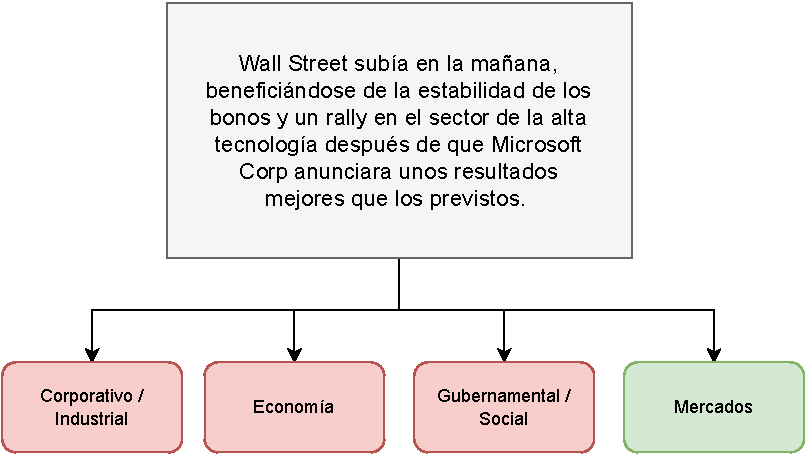
\includegraphics[scale=0.65]{images/nlp-example-document-classification.pdf}
    \caption{An example of document classification. Taken from the MLDoc \citep{schwenk-li-2018-corpus} dataset.}
    \label{fig:nlp-example-document-classification}
\end{figure}

\end{frame}
%------------------------------------------------
\begin{frame}{Motivation}

\centering
\begin{figure}
    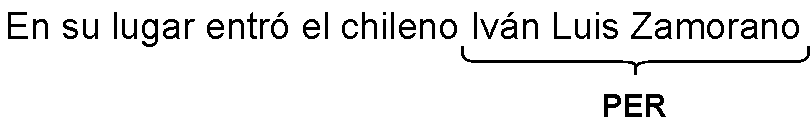
\includegraphics[scale=0.7]{images/nlp-example-ner.pdf}
    \caption{An example of named entity recognition. Taken from the CoNLL2002 NER \citep{tjong-kim-sang-2002-introduction} dataset.}
    \label{fig:nlp-example-ner}
\end{figure}

\end{frame}
%------------------------------------------------
\begin{frame}{Motivation}

\centering
\begin{figure}
    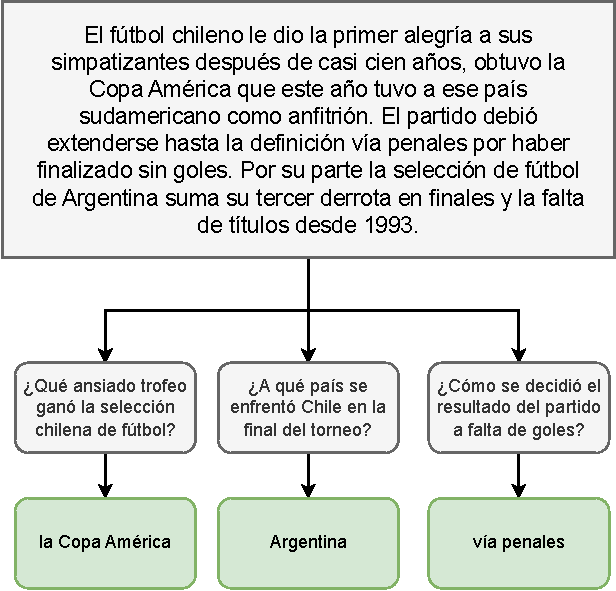
\includegraphics[scale=0.65]{images/nlp-example-question-answering.pdf}
    \caption{An example of question answering. Taken from the SQAC \citep{gutierrezfandino2022-roberta-bne} dataset.}
    \label{fig:nlp-example-question-answering}
\end{figure}

\end{frame}
%------------------------------------------------
\begin{frame}{Motivation}

\centering
\begin{figure}
    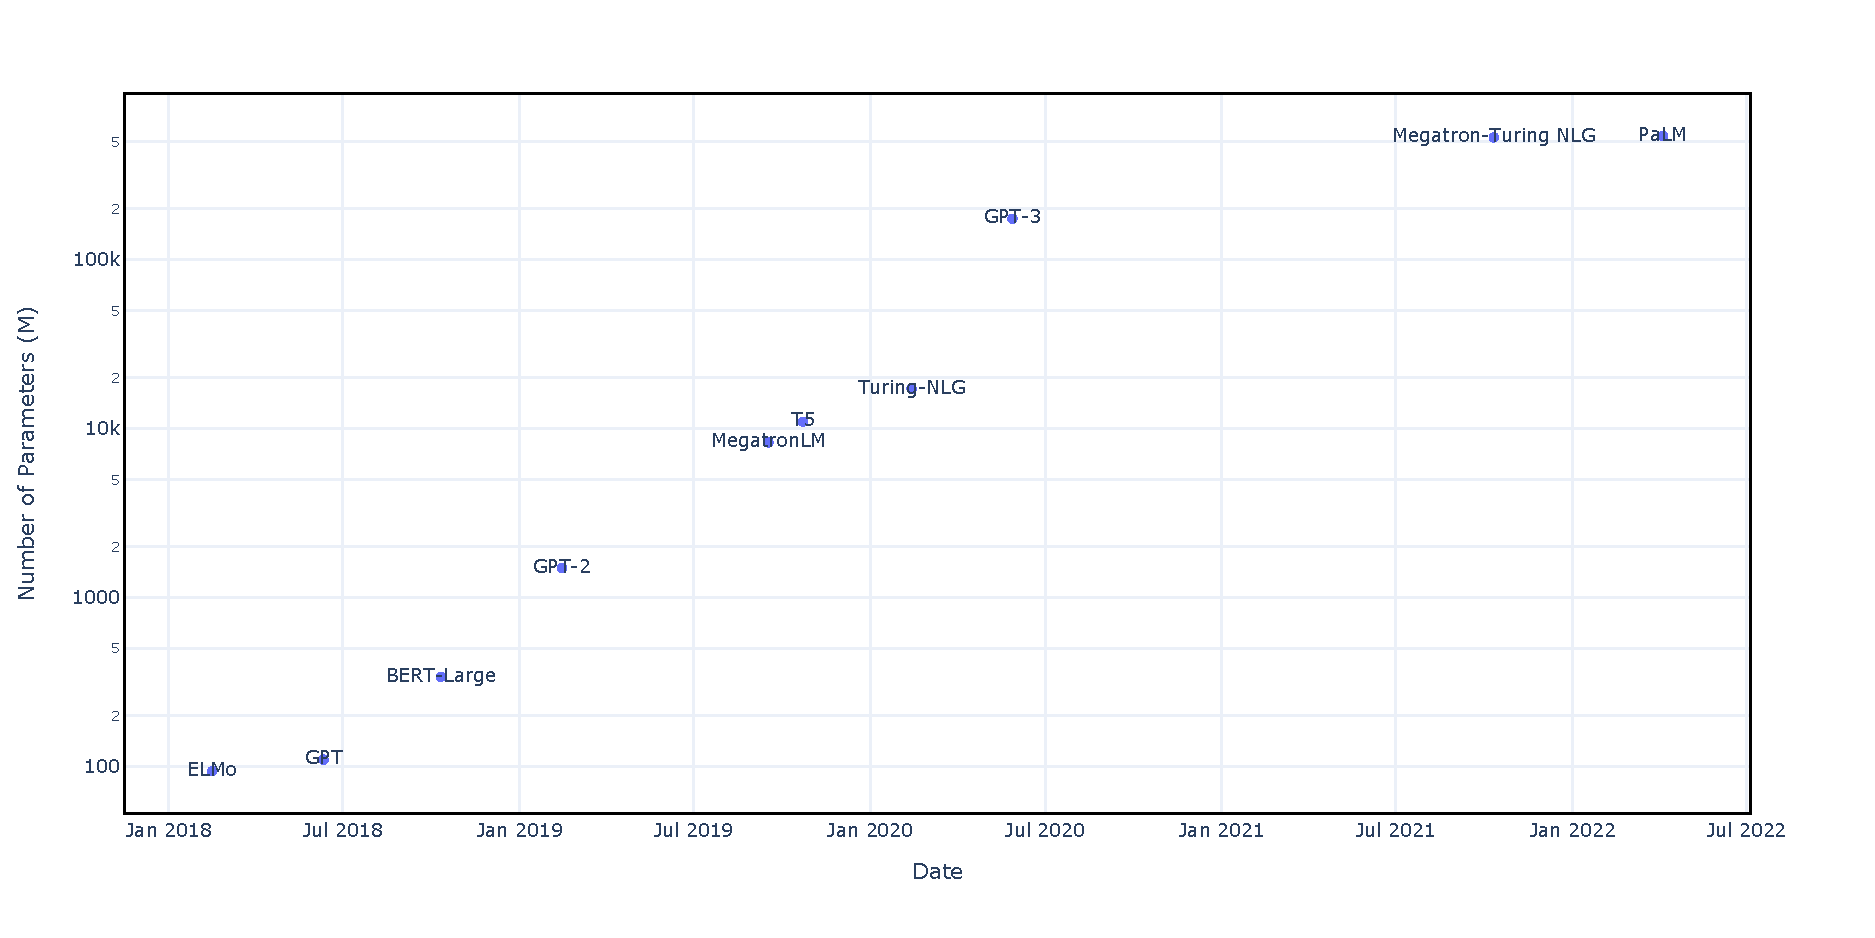
\includegraphics[width=\columnwidth]{images/llms_fig.pdf}
    % \caption{A summary of the number of parameters in various modern language models, with increasing model sizes from older to newer models. The models included in this comparison are ELMo \citep{peters-etal-2018-deep}, GPT \citep{radford2018improving}, BERT \citep{devlin-etal-2019-bert}, GPT-2 \citep{radford2019language}, MegatronLM \citep{megatron-lm}, T5 \citep{t5-raffel}, Turing-NLG \citep{rasley2020deepspeed-turingnlg}, GPT-3 \citep{brown-gpt3}, Megatron-Turing NLG \citep{megatron-turing-nlg} and PaLM \citep{palm-google}.}
    \label{fig:llms}
\end{figure}

\end{frame}
%------------------------------------------------





%------------------------------------------------
\section{Problem}
%------------------------------------------------
\begin{frame}{Problem}
\centering
\huge{As \alert{models grows} in size and computational complexity, it’s \alert{difficult} to put them in \alert{production} for real time applications or the use of them in hardware restricted devices like mobile phones.}
\end{frame}
%------------------------------------------------
\begin{frame}{Problem}
\centering
\huge{And even \alert{more difficult} for the \alert{Spanish} language because of the lack of Spanish-specific resources and models.}
\end{frame}
%------------------------------------------------







%------------------------------------------------
\section{Hypothesis and Objectives}
%------------------------------------------------
\begin{frame}{Hypothesis}
\centering
\Large{Adopting more parameter-efficient model architectures and employing knowledge distillation techniques to transfer knowledge from larger models to smaller ones can significantly enhance model compactness and inference speed, while maintaining most of the performance exhibited by larger models on Spanish NLP tasks.}
\end{frame}
%------------------------------------------------
\begin{frame}{General Objective}
\centering
\huge{To develop \alert{Spanish language models} that are more \alert{compact} and \alert{computationally efficient} while maintaining high levels of task-performance.}
\end{frame}
%------------------------------------------------
\begin{frame}{Specific Objectives}
\begin{enumerate}
    \item To measure the size and inference speed of pre-trained Spanish language models that are currently available.
    \item To develop models for the Spanish language that are more parameter-efficient by utilizing weight-shared model architectures.
    \item To train models for Spanish that are more inference-efficient by applying task-specific knowledge distillation on Spanish NLP tasks.
    \item To evaluate the mentioned techniques on a diverse set of Spanish NLP tasks.
    \item To evaluate how the model size impacts the task performance while using these techniques.
    \item To release those models publicly as a resource for further research.
\end{enumerate}
\end{frame}
%------------------------------------------------








%------------------------------------------------
\section{Background and Related Work}
%------------------------------------------------
% \begin{frame}{Background - Transformers}
% \end{frame}
%------------------------------------------------
\begin{frame}{Background - BERT}

\begin{columns}[c] % The "c" option specifies centered vertical alignment while the "t" option is used for top vertical alignment

\column{.65\textwidth}
\begin{figure}
    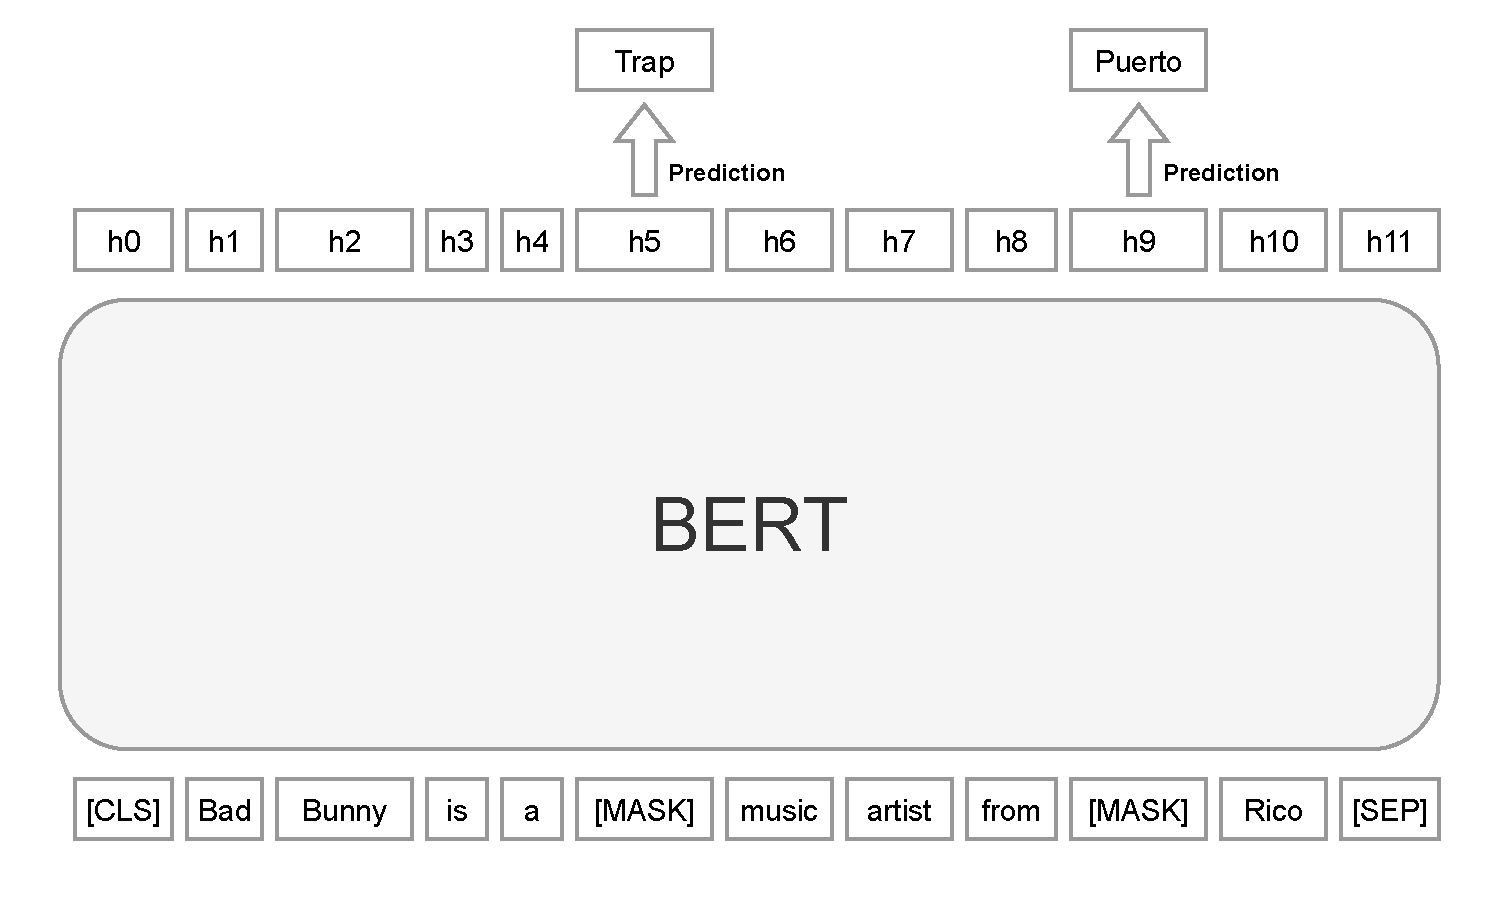
\includegraphics[width=\columnwidth]{images/BERT-MLM.pdf}
    \caption{The masked language modeling (MLM) task used by BERT as pre-training task.}
    \label{fig:bert-mlm}
\end{figure}

\column{0.35\textwidth}
\begin{itemize}
    \item Bidirectional Encoder Representations from Transformers \citep{devlin-etal-2019-bert}.
    \item Transformer-encoder.
    \item Pre-training on MLM and NSP.
    \item Fine-tuning on downstream tasks.
    \item \textit{base} (110M) and \textit{large} (330M).
\end{itemize}

\end{columns}
\end{frame}
%------------------------------------------------
% \begin{frame}{Background - RoBERTa}
% \end{frame}
%------------------------------------------------
\begin{frame}{Background - ALBERT}
\begin{columns}[c] % The "c" option specifies centered vertical alignment while the "t" option is used for top vertical alignment

\column{0.35\textwidth}
\begin{itemize}
    \item A Lite BERT \citep{albert-zhenzhong}.
    \item Transformer-encoder.
    \item Embedding factorization and Parameter-sharing.
    \item Pre-training on MLM and SOP.
    \item Fine-tuning on downstream tasks.
    \item \textit{base} (12M) to \textit{xxlarge} (235M).
\end{itemize}

\column{.65\textwidth}
\begin{figure}
    \centering
    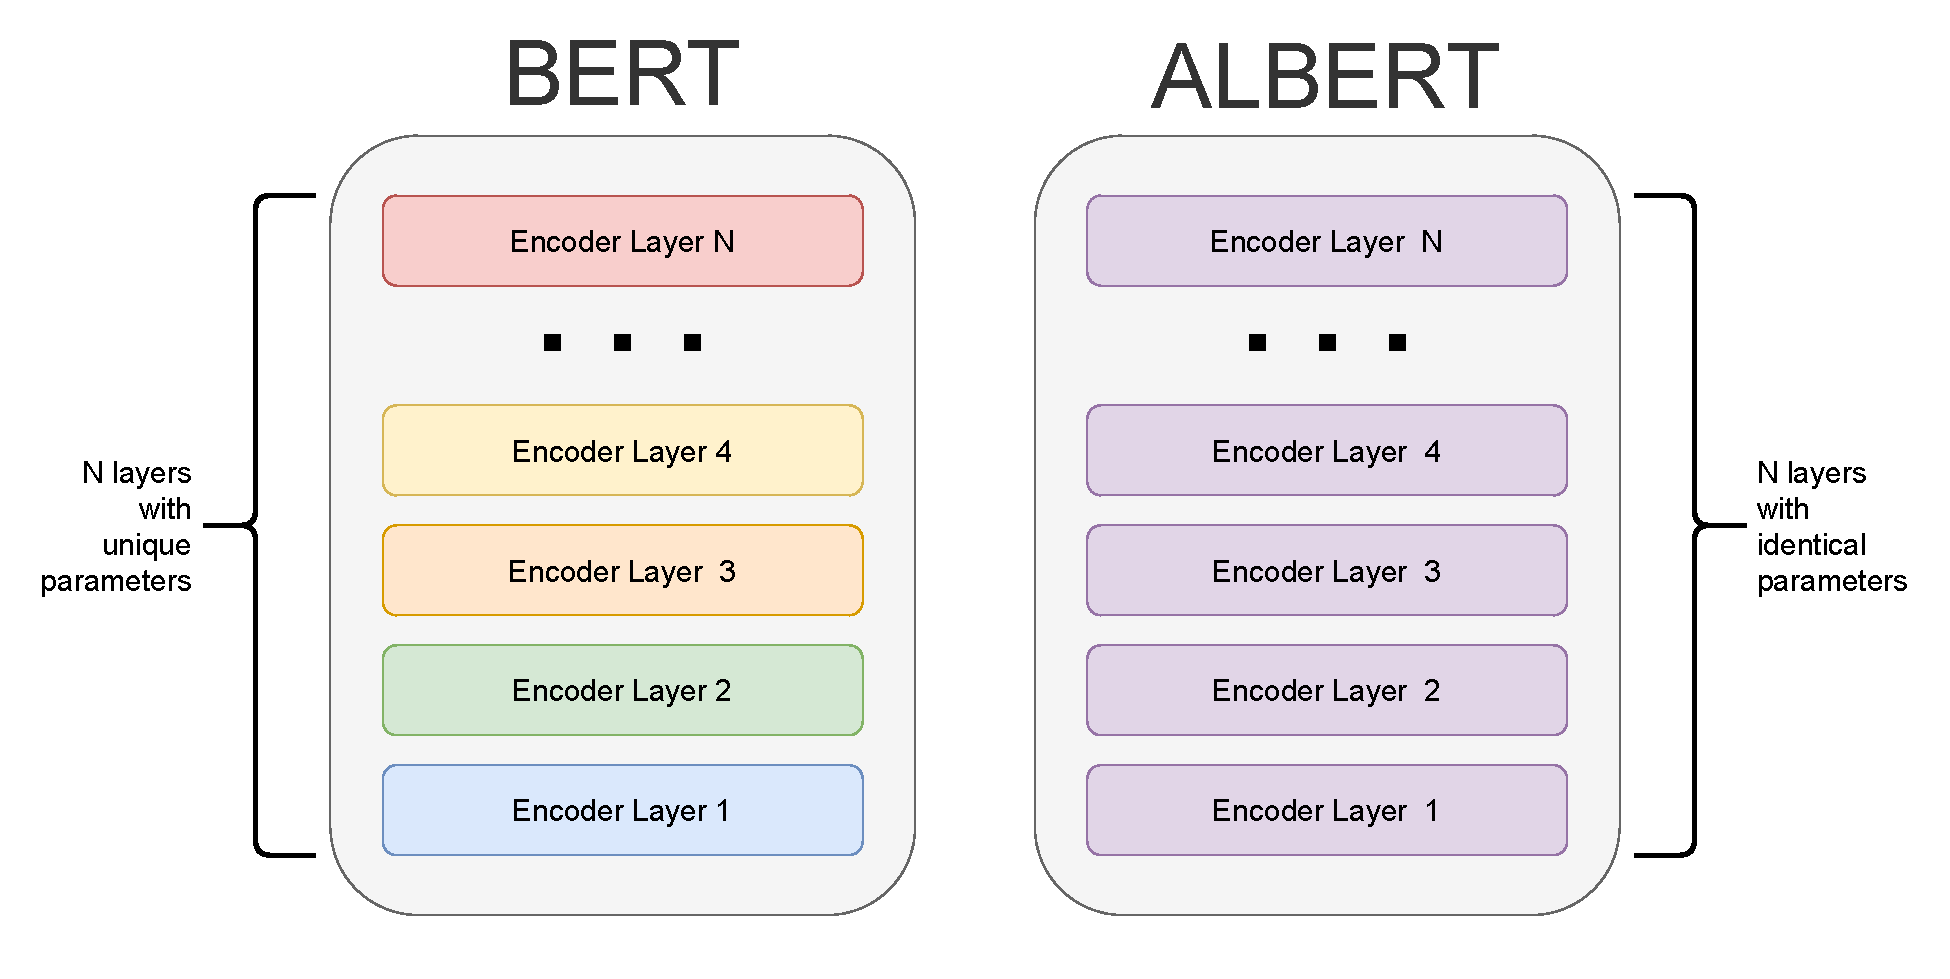
\includegraphics[width=\columnwidth]{images/bert-vs-albert-architecture.pdf}
    \caption{A design comparison of BERT and ALBERT, focusing on the parameter utilization strategy adopted by each model.}
    \label{fig:bert-vs-albert-architecture}
\end{figure}

\end{columns}
\end{frame}
%------------------------------------------------
\begin{frame}{Background - Multilingual and Monolingual Models}

\begin{wideitemize}
    \item Multilingual models:
    \begin{itemize}
        \item Models that are trained simultaneously using data from several languages.
        \item Examples: mBERT (104 languages), XLM-R (100 languages.
        \item Generally, larger vocabularies, to be able to represent all languages.
    \end{itemize}
    \item Monolingual models:
    \begin{itemize}
        \item Models trained on a single language.
        \item CamemBERT \citep{martin-etal-2020-camembert} and FlauBERT \citep{le-etal-2020-flaubert-unsupervised} for French, BERTje \citep{devries2019bertje} and RobBERT \citep{delobelle-etal-2020-robbert} for Dutch, FinBERT~\citep{virtanen2019multilingual} for Finish, BETO \citep{CaneteCFP2020} for Spanish.
        \item Generally outperform multilingual models.
    \end{itemize}
\end{wideitemize}

\end{frame}
%------------------------------------------------
\begin{frame}{Background - Compression Techniques}

\begin{wideitemize}
    \item Methods to reduce the overall size or computational complexity of a model.
    \item \textbf{Pruning}: aims to reduce the number of connections (weights) in a neural network by identifying and removing redundant connections.
    \item \textbf{Quantization}: compresses the original network by reducing the number of bits required to represent each weight.
    \item \textbf{Knowledge Distillation}: transfers the knowledge from a big model (teacher) to a smaller model (student) by training the student to imitate the teacher.
\end{wideitemize}

\end{frame}
%------------------------------------------------
\begin{frame}{Background - Knowledge Distillation}
\centering
\begin{figure}
    \includesvg[width=\columnwidth]{images/my-kd-overview.svg}
    \caption{The figure provides a visual representation of the Knowledge Distillation \citep{hinton2015distilling} framework applied in this work.}
    \label{fig:kd-overview}
\end{figure}
\end{frame}
%------------------------------------------------
\begin{frame}{Background - Knowledge Distillation}
Two models, the teacher model, say $M_T$, and a student model, say $M_S$. We train $M_S$ to imitate $M_T$. We define the distillation objective as $L_{KD}$:

$$L_{KD} = L_O(M_T(x), M_S(x))$$

Where $L_O$ is a loss function that works on the logits of $M_T$ and $M_S$. The most common choices for this loss are the cross entropy loss, the KL-divergence loss and the mean-squared error loss.

Also, we can include the gold labels from the training dataset. The complete loss, accounting these labels can be seen as:

$$L = \alpha L_{CE} + (1 - \alpha) L_{KD}$$

Where $L_{CE}$ is the traditional cross-entropy loss against gold labels and $\alpha \in [0, 1]$ defines the weight of each loss.
\end{frame}
%------------------------------------------------
\begin{frame}{Related Work}
\begin{wideitemize}
    \item \citet{tang-distilling-2019} uses KD to transfer the knowledge from BERT to lighter RNNs. 
    \item \citet{turc2019} proposes pre-training compact BERT models and then using task-specific KD to achieve better results.
    \item \citet{distilbert-sanh} introduces a task-agnostic scheme where KD is used on the pre-training task.
    \item \citet{wang-minilm} and \citet{jiao-etal-2020-tinybert} proposed different methods exclusive for Transformers, to directly distill the knowledge from the self-attention layers of the teacher model to the student model.
\end{wideitemize} 
\end{frame}
%------------------------------------------------





\section{Preliminaries: Evaluation Tasks and Baselines}
%------------------------------------------------
\begin{frame}{Evaluation Tasks}

\begin{columns}[c] % The "c" option specifies centered vertical alignment while the "t" option is used for top vertical alignment

\column{0.5\textwidth}
\begin{enumerate}
    \item \textbf{Text Classification}
    \begin{itemize}
        \item Document Classification.
        \item Natural Language Inference.
        \item Paraphrase Identification.
    \end{itemize}
\end{enumerate}

\column{.5\textwidth}
\begin{enumerate}
    \setcounter{enumi}{1}
    \item \textbf{Sequence Tagging}
    \begin{itemize}
        \item Named Entity Recognition.
        \item Part-of-Speech Tagging.
    \end{itemize}
    \item \textbf{Question Answering}
\end{enumerate}

\end{columns}

\begin{table}[]
\begin{center}
\resizebox{\columnwidth}{!}{
\begin{tabular}{lccccc}
\hline
Dataset Name        & Task Type                & Number of Categories & Train Size & Validation Size & Test Size \\ \hline
MLDoc \citep{schwenk-li-2018-corpus}       & Text Classification & 4                    & 9458       & 1000            & 4000      \\
PAWS-X \citep{yang-etal-2019-paws}      & Text Classification & 2                    & 49401      & 2000            & 2000      \\
XNLI \citep{conneau-etal-2018-xnli}       & Text Classification & 3                    & 392702     & 2490            & 5010      \\
POS \citep{taule-etal-2008-ancora}        & Sequence Tagging    & 18                   & 14305      & 1654            & 1721      \\
NER \citep{tjong-kim-sang-2002-introduction}        & Sequence Tagging    & 9                    & 8324       & 1916            & 1518      \\
MLQA \citep{lewis-etal-2020-mlqa}        & Question Answering  & -                    & 81810      & 500             & 5253      \\
SQAC \citep{gutierrezfandino2022-roberta-bne}        & Question Answering  & -                    & 15036      & 1864            & 1910      \\
TAR / XQuAD \citep{carrino-etal-2020-automatic, artetxe-etal-2020-cross} & Question Answering  & -                    & 87595      & 10570           & 1190      \\ \hline
\end{tabular}}
\end{center}
\caption{Details of the datasets used to evaluate our proposed models.}
\label{table:dataset-statistics}
\end{table}
\end{frame}
%------------------------------------------------
\begin{frame}{Inference Metrics}
\textbf{Metrics}
\begin{itemize}
    \item Size: Number of Parameters.
    \item Speed: Multiply-accumulate Operations (MACs).
\end{itemize}

\vspace{0.5cm}

\textbf{Conditions}
\begin{itemize}
    \item Batch size = 1.
    \item Max. sequence length = 512.
\end{itemize}
\end{frame}
%------------------------------------------------
\begin{frame}{Pre-trained Models for Spanish}
\textbf{Aim}
\begin{itemize}
    \item Include all publicly available Transformer-encoder based models trained on Spanish general domain corpora as baselines.
\end{itemize}

\begin{table}[]
\begin{center}
\resizebox{\columnwidth}{!}{
\begin{tabular}{lccccccccc}
\hline
\textbf{Model Name} & \textbf{Architecture} & \textbf{Size} & \textbf{Vocab Size} & \textbf{Vocab Types}  & \textbf{Max Seq Length} & \textbf{Parameters} & \textbf{Domain} & \textbf{Availability} & \textbf{Reference} \\ \hline
\multicolumn{10}{c}{Included}                                                                                                                                                                                                                               \\ \hline
BETO                & BERT                  & base                & 32K                      & uncased, cased             & 512                          & 110M                          & General         & Public                &     \citep{CaneteCFP2020}                    \\
DistilBETO          & DistilBERT            & base                & 32K                      & uncased                    & 512                          & 67M                           & General         & Public                &      \citep{donoso2021entrenamiento}          \\
RoBERTa-BNE base    & RoBERTa               & base                & 50K                      & cased                      & 514                          & 125M                          & General         & Public                &      \citep{gutierrezfandino2022-roberta-bne} \\
RoBERTa-BNE large   & RoBERTa               & large               & 50K                      & cased                      & 514                          & 355M                          & General         & Public                &      \citep{gutierrezfandino2022-roberta-bne} \\
BERTIN              & RoBERTa               & base                & 50K                      & cased                      & 514                          & 125M                          & General         & Public                &      \citep{BERTIN}                           \\ \hline
\multicolumn{10}{c}{Not Included}                                                                                                                                                                                                                           \\ \hline
GPT-2-BNE base      & GPT-2                 & base                & 50K                      & cased                      & 512                          & 124M                          & General         & Public                &      \citep{gutierrezfandino2022-roberta-bne} \\
GPT-2-BNE large     & GPT-2                 & large               & 50K                      & cased                      & 512                          & 773M                          & General         & Public                &
\citep{gutierrezfandino2022-roberta-bne} \\
RigoBERTa           & DeBERTa               & base                & 50K                      & -                          & 512                          & -                             & General         & Private               & 
\citep{serrano2022rigoberta}             \\
RoBERTuito          & RoBERTa               & base                & 30K                      & uncased, cased, deaccented & 130                          & 109M                          & Social Media    & Public                &      \citep{perez-etal-2022-robertuito}       \\
BSC-Bio             & RoBERTa               & base                & 50K                      & cased                      & 514                          & 125M                          & Biomedical      & Public                &      \citep{carrino-etal-2022-pretrained}     \\
RoBERTalex          & RoBERTa               & base                & 52K                      & cased                      & 514                          & 126M                          & Legal           & Public                &      \citep{gutierrezfandino2021legal}        \\
Longformer-BNE      & Longformer            & base                & 50K                      & cased                      & 4098                         & 149M                          & General         & Public                &      -                      \\ \hline
\end{tabular}}
\end{center}
\caption{Summary of pre-trained Transformer models for Spanish.}
\label{table:summary-spanish-models}
\end{table}

\end{frame}
%------------------------------------------------

%------------------------------------------------
\section{Proposed Spanish NLP Resources: ALBETO and Speedy Gonzales}
%------------------------------------------------
%\subsection{ALBETO: Light Models for Spanish}
%------------------------------------------------
\begin{frame}{ALBETO: Light models for Spanish}
\centering
\large{ALBETO: a series of 5 lightweight models that follow the ALBERT architecture and are pre-trained exclusively on Spanish corpora with sizes that range from 5M to 223M of parameters.}
\end{frame}
%------------------------------------------------
\begin{frame}{ALBETO: Model Architecture}

\begin{itemize}
    \item ALBERT architecture.
    \item 31K lowercase subword tokens.
\end{itemize}

\begin{table}[]
\begin{center}
\begin{tabular}{lcccc}
\hline
\textbf{Model}          & \textbf{Parameters} & \textbf{Layers} & \textbf{Hidden} & \textbf{Embedding} \\ \hline
ALBETO \textit{tiny}    & 5M         & 4      & 312    & 128       \\ 
ALBETO \textit{base}    & 12M        & 12     & 768    & 128       \\ 
ALBETO \textit{large}   & 18M        & 24     & 1024   & 128       \\ 
ALBETO \textit{xlarge}  & 59M        & 24     & 2048   & 128       \\ 
ALBETO \textit{xxlarge} & 223M       & 12     & 4096   & 128       \\ \hline
\end{tabular}
\end{center}
\caption{The configurations of each ALBETO model trained in this work.}
\label{table:albeto-configurations}
\end{table}

\end{frame}
%------------------------------------------------
\begin{frame}{ALBETO: Training Process}

\begin{figure}
    \centering
    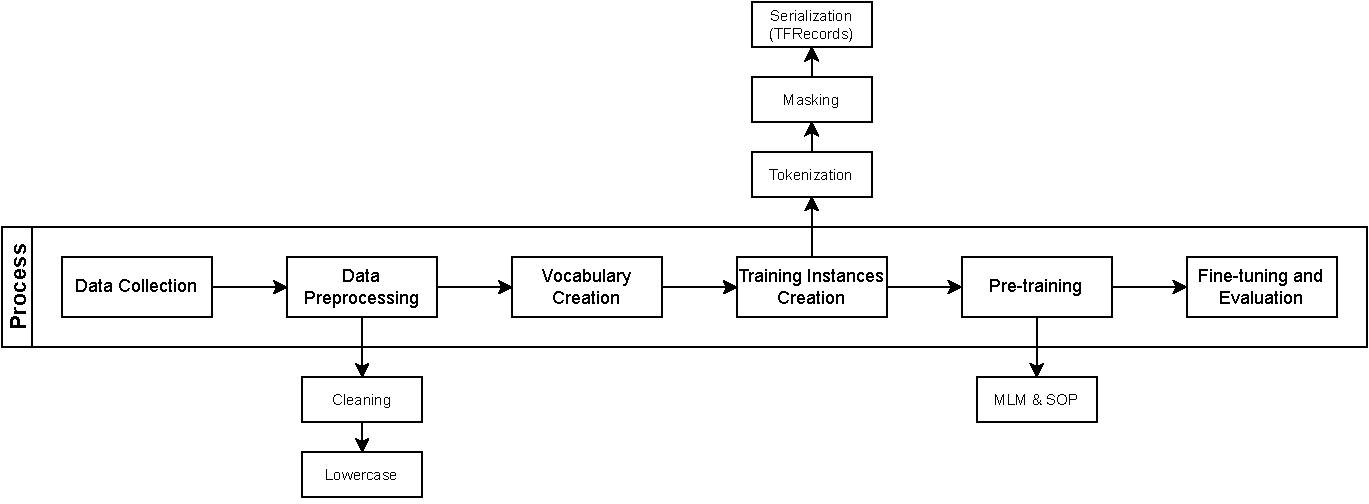
\includegraphics[width=\columnwidth]{images/ALBETO-training-process-diagram.pdf}
    \caption{A broad overview of the process involved in the creation of ALBETO models. Sub-processes relevant to distinct stages are portrayed outside the main frame.}
    \label{fig:ALBETO-training-process-diagram}
\end{figure}

\end{frame}
%------------------------------------------------
\begin{frame}{ALBETO: Evaluation}

\begin{wideitemize}
    \item Fine-tuning on downstream tasks.
    \item Tasks: text classification, sequence tagging and question answering.
    \item Hyperparameter search:
    \begin{itemize}
        \item All models:
        \begin{itemize}
            \item Batch size: 16, 32, 64.
            \item Epochs: 2, 3, 4.
        \end{itemize}
        \item BETO, DistilBETO, RoBERTa-BNE, BERTIN, ALBETO \textit{tiny} and \textit{base}:
        \begin{itemize}
            \item Learning rate: 1e-5, 2e-5, 3e-5, 5e-5.
        \end{itemize}
        \item ALBETO \textit{large}, \textit{xlarge} and \textit{xxlarge}:
        \begin{itemize}
            \item Learning rate: 1e-6, 2e-6, 3e-6, 5e-6.
        \end{itemize}
    \end{itemize}
\end{wideitemize}

\end{frame}
%------------------------------------------------









%------------------------------------------------
%\subsection{Speedy Gonzales: Fast Models for Spanish}
%------------------------------------------------
\begin{frame}{Speedy Gonzales: Fast Models for Spanish}
\centering
\large{Speedy Gonzales: a collection of fast task-specific language models based on ALBETO, which were trained using Task-specific Knowledge Distillation.}
\end{frame}
%------------------------------------------------
\begin{frame}{Speedy Gonzales: Approach}

\begin{figure}
    \centering
    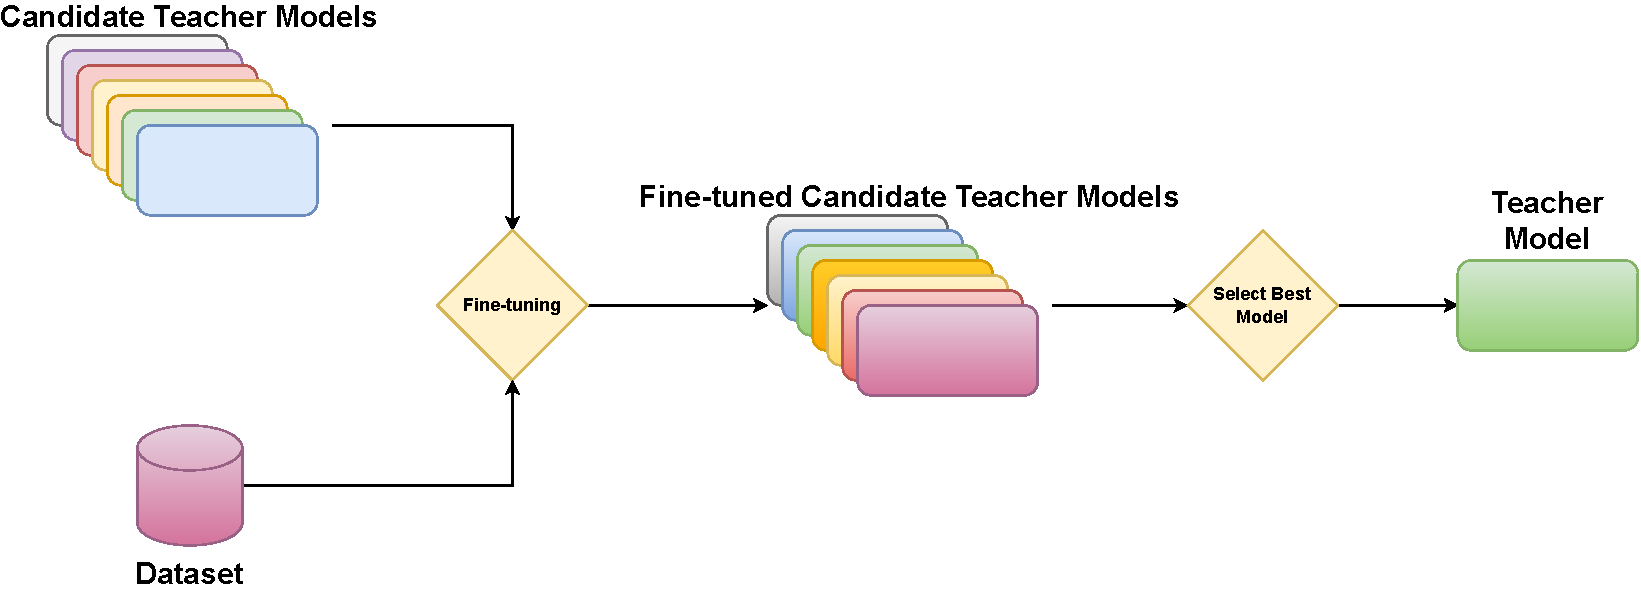
\includegraphics[width=\columnwidth]{images/KD-approach-single-dataset-first-stage.pdf}
    \caption{The first stage of our approach, which involves fine-tuning a set of candidate models on a specific dataset, followed by the selection of the best-performing model as the teacher model for that dataset.}
    \label{fig:KD-approach-single-dataset-first-stage}
\end{figure}

\end{frame}
%------------------------------------------------
\begin{frame}{Speedy Gonzales: Approach}

\begin{figure}
    \centering
    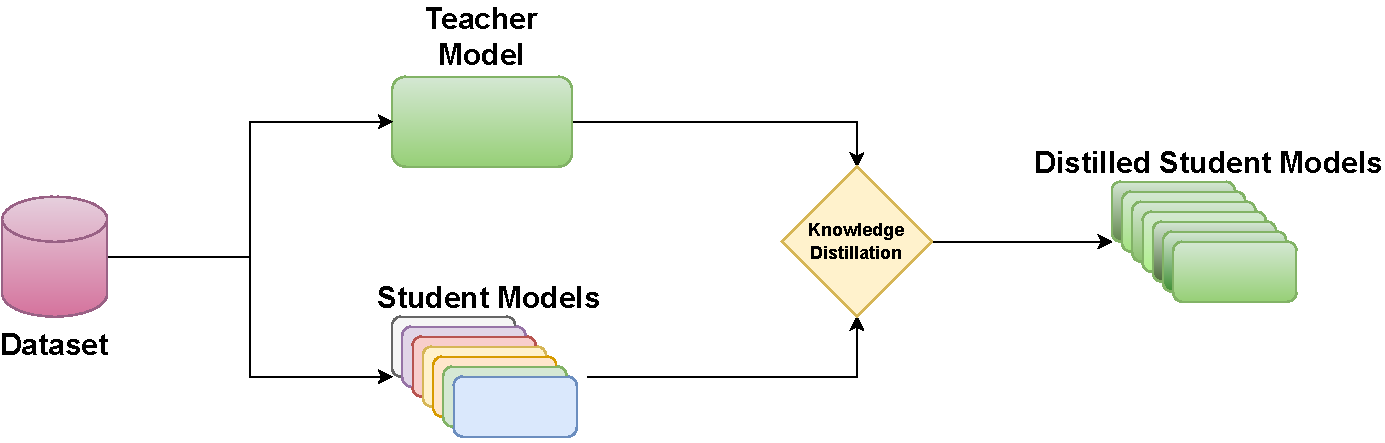
\includegraphics[width=\columnwidth]{images/KD-approach-single-dataset-second-stage.pdf}
    \caption{The second stage of our approach, which employs the selected teacher model to train a set of student models using knowledge distillation.}
    \label{fig:KD-approach-single-dataset-second-stage}
\end{figure}

\end{frame}
%------------------------------------------------
\begin{frame}{Speedy Gonzales: Approach}

\textbf{Candidate teacher models:}
\begin{itemize}
    \item All publicly available Transformer-encoder based models trained on Spanish general domain corpora.
    \item BETO, DistilBETO, RoBERTa-BNE, BERTIN and ALBETO.
\end{itemize}

\vspace{0.5cm}

\textbf{Student models:}
\begin{itemize}
    \item ALBETO \textit{tiny}.
    \item A collection of faster models based on ALBETO \textit{base}:
    \begin{itemize}
        \item Models that follows the ALBETO \textit{base} configuration, but with less layers.
        \item Noted as ALBETO \textit{base-n}, $n \in (2, 4, 6, 8, 10)$.
    \end{itemize}
\end{itemize}

\end{frame}
%------------------------------------------------
\begin{frame}{Speedy Gonzales: Evaluation}

\textbf{First stage:}
\begin{itemize}
    \item Same as ALBETO evaluation.
    \item Selected best teacher models.
\end{itemize}

\textbf{Second stage:}
\begin{itemize}
    \item Task-specific Knowledge Distillation on downstream tasks.
    \item Tasks: text classification, sequence tagging and question answering.
    \item KL-Divergence loss, $\alpha = 0$ and $T = 1$. 
    \item Cached teacher predictions.
    \item Hyperparameter search:
    \begin{itemize}
        \item Batch size: 16, 32, 64.
        \item Learning rate: 5e-5, 1e-4.
        \item Epochs: 50.
        \item Early stopping with tolerance of 10 epochs of no improving.
    \end{itemize}
\end{itemize}

\end{frame}
%------------------------------------------------









%------------------------------------------------
\section{Results and Discussion}
%------------------------------------------------
\begin{frame}{Task Performance - Text Classification}

\begin{table}[]
\begin{center}
\resizebox{0.4\columnwidth}{!}{
\begin{tabular}{lccc}
\hline
\textbf{Model}    & \textbf{MLDoc} & \textbf{PAWS-X} & \textbf{XNLI}  \\ \hline
\multicolumn{4}{c}{Fine-tuning}                                       \\ \hline
BETO uncased      & 96.38          & 84.25           & 77.76          \\
BETO cased        & 96.65          & 89.80           & 81.98          \\
DistilBETO        & 96.35          & 75.80           & 76.59          \\
ALBETO tiny       & 95.82          & 80.20           & 73.43          \\
ALBETO base       & 96.07          & 87.95           & 79.88          \\
ALBETO large      & 92.22          & 86.05           & 78.94          \\
ALBETO xlarge     & 95.70          & 89.05           & 81.68          \\
ALBETO xxlarge    & 96.85          & 89.85           & \textbf{82.42} \\
BERTIN            & 96.47          & 88.65           & 80.50          \\
RoBERTa BNE base  & 96.82          & 89.90           & 81.12          \\
RoBERTa BNE large & \textbf{97.00} & \textbf{90.00}  & 51.62          \\ \hline
\multicolumn{4}{c}{Task-specific Knowledge Distillation}              \\ \hline
ALBETO tiny       & 96.40          & 85.05           & 75.99          \\
ALBETO base-2     & 96.20          & 76.75           & 73.65          \\
ALBETO base-4     & 96.35          & 86.40           & 78.68          \\
ALBETO base-6     & 96.40          & 88.45           & 81.66          \\
ALBETO base-8     & 96.70          & 89.75           & \textbf{82.55} \\
ALBETO base-10    & \textbf{96.88} & \textbf{89.95}  & 82.26          \\ \hline
\end{tabular}}
\end{center}
\caption{Models evaluated on sentence or two sentences classification tasks, results are measured using accuracy on the test set of each dataset.}
\label{table:results-mldoc-pawsx-xnli}
\end{table}

\end{frame}
%------------------------------------------------
\begin{frame}{Task Performance - Sequence Tagging}

\begin{table}[]
\begin{center}
\resizebox{0.3\columnwidth}{!}{
\begin{tabular}{lcc}
\hline
\textbf{Model}      & \textbf{POS}     & \textbf{NER}    \\ \hline
\multicolumn{3}{c}{Fine-tuning}                          \\ \hline
BETO uncased        & 97.81            & 80.85           \\
BETO cased          & 98.95            & \textbf{87.14}  \\
DistilBETO          & 97.67            & 78.13           \\
ALBETO tiny         & 97.34            & 75.42           \\
ALBETO base         & 98.21            & 82.89           \\
ALBETO large        & 97.98            & 82.36           \\
ALBETO xlarge       & 98.43            & 83.06           \\
ALBETO xxlarge      & 98.43            & 83.06           \\
BERTIN              & \textbf{99.02}   & 85.66           \\
RoBERTa BNE base    & 99.00            & 86.80           \\
RoBERTa BNE large   & 61.83            & 21.47           \\ \hline
\multicolumn{3}{c}{Task-specific Knowledge Distillation} \\ \hline
ALBETO tiny         & 97.36            & 72.51           \\
ALBETO base-2       & 97.17            & 69.69           \\
ALBETO base-4       & 97.60            & 74.58           \\
ALBETO base-6       & 97.82            & 78.41           \\
ALBETO base-8       & 97.96            & 80.23           \\
ALBETO base-10      & \textbf{98.00}   & \textbf{81.10}  \\ \hline
\end{tabular}}
\end{center}
\caption{Models evaluated on sequence tagging tasks, results are measured using the F1 Score on the test set of each dataset.}
\label{table:results-pos-ner}
\end{table}

\end{frame}
%------------------------------------------------
\begin{frame}{Task Performance - Question Answering}

\begin{table}[]
\begin{center}
\resizebox{0.55\columnwidth}{!}{
\begin{tabular}{lccc}
\hline
\textbf{Model}    & \textbf{MLQA}          & \textbf{SQAC} & \textbf{TAR, XQuAD}    \\ \hline
\multicolumn{4}{c}{Fine-tuning}                                                     \\ \hline
BETO uncased      & 64.12 / 40.83          & 72.22 / 53.45 & 74.81 / 54.62          \\
BETO cased        & 67.65 / 43.38          & 78.65 / 60.94 & 77.81 / 56.97          \\
DistilBETO        & 57.97 / 35.50          & 64.41 / 45.34 & 66.97 / 46.55          \\
ALBETO tiny       & 51.84 / 28.28          & 59.28 / 39.16 & 66.43 / 45.71          \\
ALBETO base       & 66.12 / 41.10          & 77.71 / 59.84 & 77.18 / 57.05          \\
ALBETO large      & 65.56 / 40.98          & 76.36 / 56.54 & 76.72 / 56.21          \\
ALBETO xlarge     & 68.26 / 43.76          & 78.64 / 59.26 & \textbf{80.15 / 59.66} \\
ALBETO xxlarge    & \textbf{70.17} / \textbf{45.99}          & \textbf{81.49} / 62.67 & 79.13 / 58.40          \\
BERTIN            & 66.06 / 42.16          & 78.42 / 60.05 & 77.05 / 57.14          \\
RoBERTa BNE base  & 67.31 / 44.50          & 80.53 / \textbf{62.72} & 77.16 / 55.46          \\
RoBERTa BNE large & 67.69 / 44.88          & 80.41 / 62.14 & 77.34 / 56.97          \\ \hline
\multicolumn{4}{c}{Task-specific Knowledge Distillation}                            \\ \hline
ALBETO tiny       & 54.17 / 32.22          & 63.03 / 43.35 & 67.47 / 46.13          \\
ALBETO base-2     & 48.62 / 26.17          & 58.40 / 39.00 & 63.41 / 42.35          \\
ALBETO base-4     & 62.19 / 38.28          & 71.41 / 52.87 & 73.31 / 52.43          \\
ALBETO base-6     & 66.35 / 42.01          & 76.99 / 59.00 & 75.59 / \textbf{56.72}          \\
ALBETO base-8     & 67.39 / 42.94          & 77.79 / 59.63 & 77.89 / \textbf{56.72}          \\
ALBETO base-10    & \textbf{68.29} / \textbf{44.29}          & \textbf{79.89} / \textbf{62.04} & \textbf{78.21} / 56.21          \\ \hline
\end{tabular}}
\end{center}
\caption{Models evaluated on question answering datasets, results are noted as F1 Score / Exact Match on the test set of each dataset.}
\label{table:results-qa}
\end{table}

\end{frame}
%------------------------------------------------
\begin{frame}{Model Efficiency and Inference Speed}

\centering
\begin{figure}
    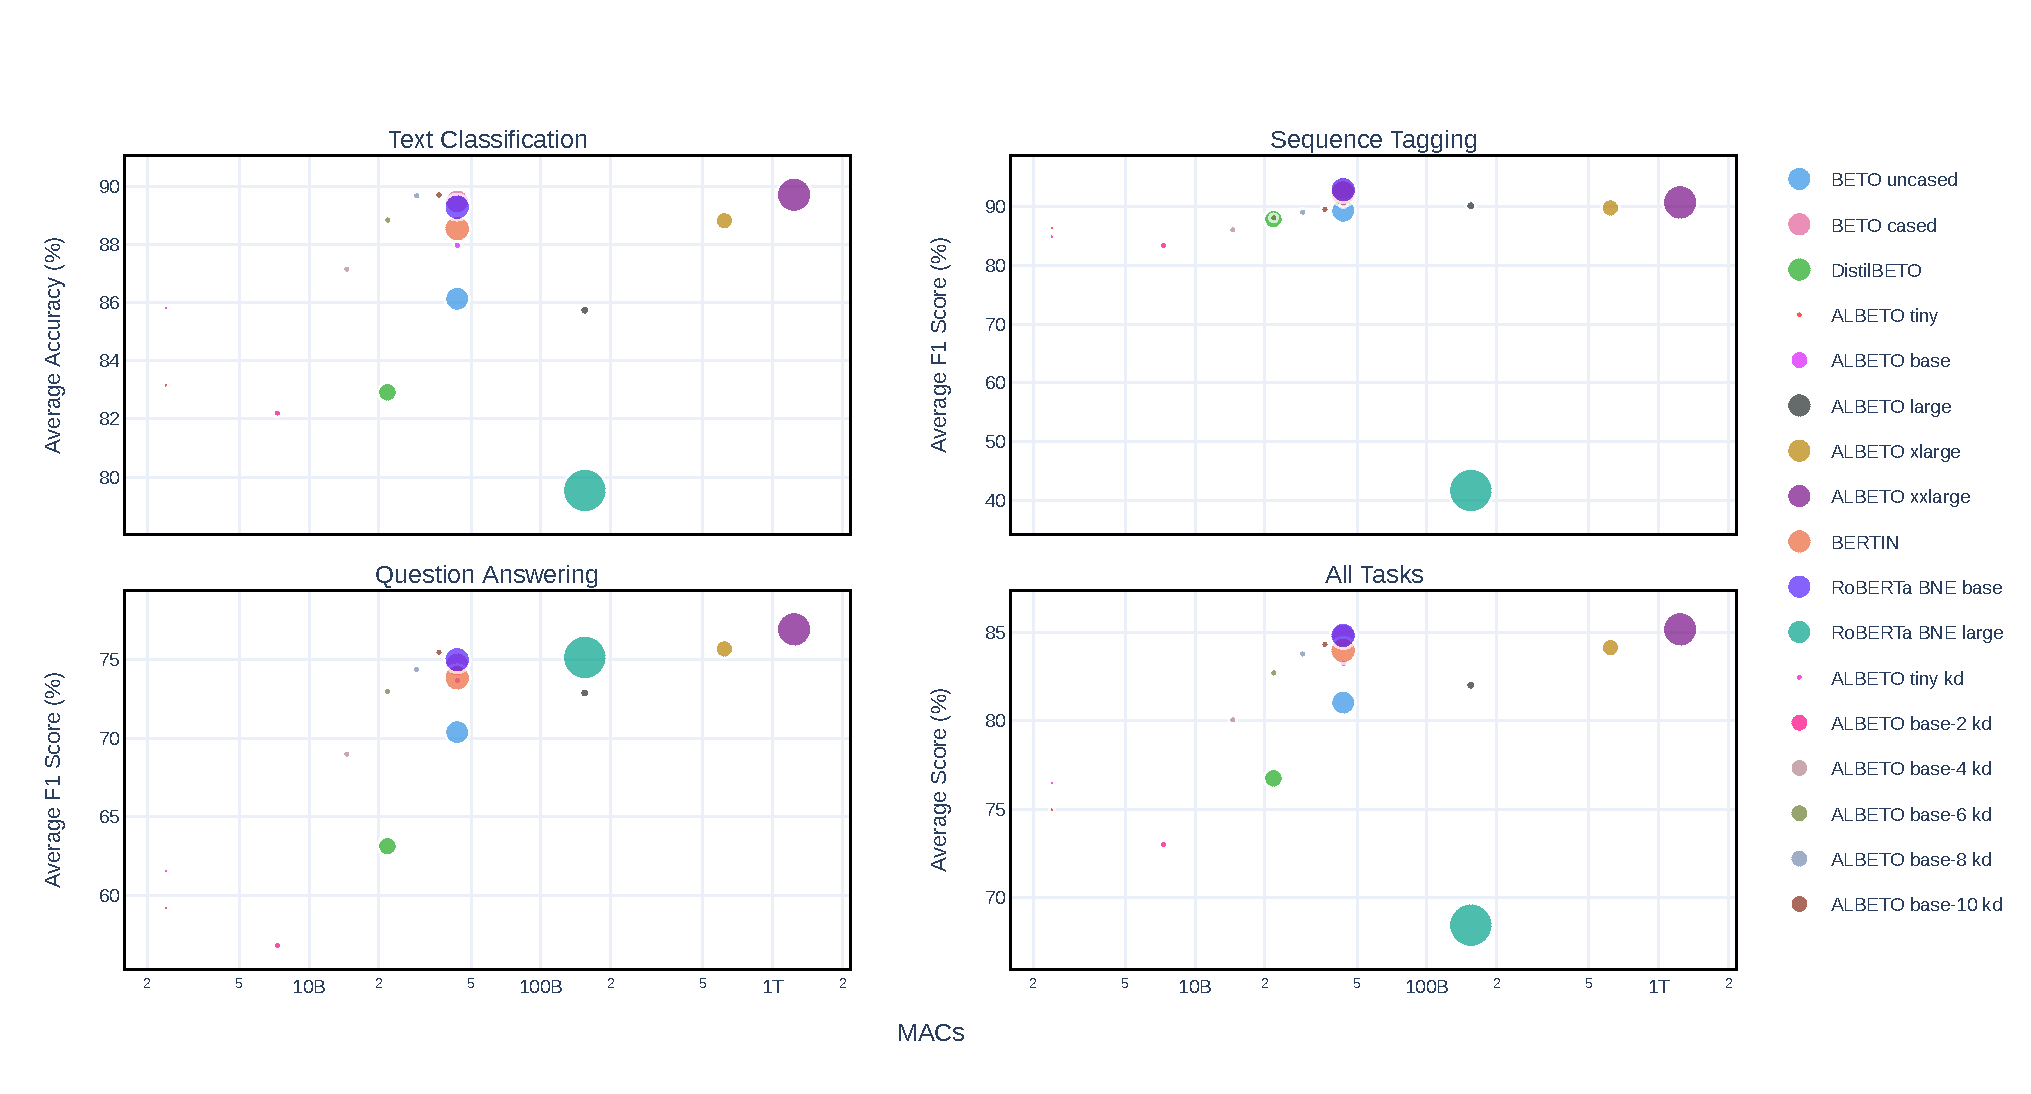
\includegraphics[width=0.95\columnwidth]{images/plot-avg-macs.pdf}
    \caption{Average of performance in the different tasks. The size of the points represents the size of the model (the number of parameters).}
    \label{fig:avg-macs-tasks}
\end{figure}

\end{frame}
%------------------------------------------------
\begin{frame}{Inference Speed on Common Hardware}

\begin{table}[]
\begin{center}
\resizebox{0.35\columnwidth}{!}{
\begin{tabular}{lcc}
\hline
\multicolumn{1}{c}{\multirow{2}{*}{\textbf{Model}}} & \multicolumn{2}{c}{Inferences per second} \\
\multicolumn{1}{c}{}                                & \textbf{CPU}        & \textbf{GPU}        \\ \hline
\multicolumn{3}{c}{Fine-tuning}                                                                 \\ \hline
BETO \textit{uncased}                                        & 3.96                & 107.19              \\
BETO \textit{cased}                                          & 4.26                & 109.02              \\
DistilBETO                                          & 9.12                & 217.40              \\
ALBETO \textit{tiny}                                         & 32.53               & 539.61              \\
ALBETO \textit{base}                                         & 4.50                & 108.62              \\
ALBETO \textit{large}                                        & 1.29                & 33.62               \\
ALBETO \textit{xlarge}                                       & 0.35                & 11.72               \\
ALBETO \textit{xxlarge}                                      & 0.14                & 6.60                \\
BERTIN                                              & 3.99                & 109.39              \\
RoBERTa BNE \textit{base}                                    & 3.82                & 107.77              \\
RoBERTa BNE \textit{large}                                   & 1.18                & 33.65               \\ \hline
\multicolumn{3}{c}{Task-specific Knowledge Distillation}                                        \\ \hline
ALBETO \textit{tiny}                                         & 32.53               & 539.61              \\
ALBETO \textit{base-2}                                       & 31.08               & 625.30              \\
ALBETO \textit{base-4}                                       & 15.16               & 319.32              \\
ALBETO \textit{base-6}                                       & 10.45               & 213.53              \\
ALBETO \textit{base-8}                                       & 6.82                & 160.66              \\
ALBETO \textit{base-10}                                      & 6.01                & 128.38              \\ \hline
\end{tabular}}
\end{center}
\caption{The number of inferences per second of models on two different hardware settings, CPU and GPU.}
\label{table:inferences-per-second}
\end{table}

\end{frame}
%------------------------------------------------
\begin{frame}{Results - Summary}

\begin{table}[]
\begin{center}
\resizebox{0.4\columnwidth}{!}{
\begin{tabular}{lccc}
\hline
\textbf{Model}    & \textbf{Parameters} & \textbf{Speedup} & \textbf{Score} \\ \hline
\multicolumn{4}{c}{Fine-tuning}                                             \\ \hline
BETO \textit{uncased}      & 110M                & 1.00x            & 81.02          \\
BETO \textit{cased}        & 110M                & 1.00x            & 84.82          \\
DistilBETO        & 67M                 & 2.00x            & 76.73          \\
ALBETO \textit{tiny}       & \textbf{5M}         & \textbf{18.05x}  & 74.97          \\
ALBETO \textit{base}       & 12M                 & 0.99x            & 83.25          \\
ALBETO \textit{large}      & 18M                 & 0.28x            & 82.02          \\
ALBETO \textit{xlarge}     & 59M                 & 0.07x            & 84.13          \\
ALBETO \textit{xxlarge}    & 223M                & 0.03x            & \textbf{85.17} \\
BERTIN            & 125M                & 1.00x            & 83.97          \\
RoBERTa BNE \textit{base}  & 125M                & 1.00x            & 84.83          \\
RoBERTa BNE \textit{large} & 355M                & 0.28x            & 68.42          \\ \hline
\multicolumn{4}{c}{Task-specific Knowledge Distillation}                    \\ \hline
ALBETO \textit{tiny}       & \textbf{5M}         & \textbf{18.05x}  & 76.49          \\
ALBETO \textit{base-2}     & 12M                 & 5.96x            & 72.98          \\
ALBETO \textit{base-4}     & 12M                 & 2.99x            & 80.06          \\
ALBETO \textit{base-6}     & 12M                 & 1.99x            & 82.70          \\
ALBETO \textit{base-8}     & 12M                 & 1.49x            & 83.78          \\
ALBETO \textit{base-10}    & 12M                 & 1.19x            & \textbf{84.32} \\ \hline
\end{tabular}}
\end{center}
\caption{The summary of results of every evaluated model in terms of parameters, inference speedup and overall score across tasks. The speedup is relative to BETO models. The score column shows the average of the metrics on all tasks.}
\label{table:results-summary}
\end{table}

\end{frame}
%------------------------------------------------




%------------------------------------------------
\section{Conclusions}
%------------------------------------------------
\begin{frame}{Summary of Contributions}
\centering
\Large{We introduced ALBETO and Speedy Gonzales, which are \alert{two novel resources} for the \alert{Spanish NLP} community that were created to \alert{improve} two key aspects of machine learning models, namely \alert{model size} and \alert{inference speed}.}

\end{frame}
%------------------------------------------------
\begin{frame}{Summary of Contributions}

\textbf{ALBETO:}
\begin{wideitemize}
    \item Language models that were pre-trained exclusively for the Spanish language, with five different sizes: \textit{tiny}, \textit{base}, \textit{large}, \textit{xlarge}, and \textit{xxlarge}.
    \item Successfully utilize the weight-shared strategy to achieve greater efficiency in terms of model parameters.
    \item The \textit{base} model, which is an \textit{uncased} model, outperforms the \textit{uncased} version of BETO while having significantly less parameters and is marginally inferior to other \textit{base}-sized models with a \textit{cased} vocabulary.
    \item The \textit{xxlarge} model outperforms all other models.
\end{wideitemize}

\end{frame}
%------------------------------------------------
\begin{frame}{Summary of Contributions}

\textbf{Speedy Gonzales:}
\begin{itemize}
    \item Collection of fast task-specific models trained using Task-specific KD.
    \item Task-Specific KD is effective in transferring knowledge from a larger model to a lighter and faster model.
    \item Speedy Gonzales models achieve comparable task performance to most base-sized models while exhibiting enhanced inference speed.
    \item There exists a trade-off between inference-efficiency of the model and task performance, as observed in the evaluation of the Speedy Gonzales models derived from the ALBETO \textit{base} model.
    \item Some tasks benefit from the use of larger and more computationally complex models (e.g. QA), while other tasks can be effectively handled by lighter and faster models (e.g. POS, MLDoc).
\end{itemize}

\end{frame}
%------------------------------------------------
\begin{frame}{Limitations and Future Research Directions}

\begin{wideitemize}
    \item We only evaluated our models on a limited set of tasks.
    \item Our KD method can be further improved to produce more efficient task-specific language models:
    \begin{itemize}
        \item Explore alternative KD approaches, such as distilling intermediate layers of the teacher model, in addition to its output.
        \item A multi-teacher approach could be studied, in which the models learn from a collection of teacher models rather than just one.
        \item Combine with other compression techniques, such as parameter-pruning or quantization.
    \end{itemize}
    \item There exists a trade-off between model size, inference speed, and task performance, making it challenging to choose an appropriate model without context. It is important to develop metrics to formally assess the this balance.
\end{wideitemize}

\end{frame}
%------------------------------------------------
\begin{frame}{Outcomes}

\textbf{Two publications:}
\begin{enumerate}
    \item ALBETO and DistilBETO: Lightweight Spanish Language Models
    \begin{itemize}
        \item \citet{canete-etal-2022-albeto}
        \item Proceedings of the 13th Edition of The Language Resources and Evaluation Conference (LREC), Marseille, France.
        \item \href{https://aclanthology.org/2022.lrec-1.457/}{\color{blue}{Paper}}, \href{https://github.com/dccuchile/lightweight-spanish-language-models}{\color{blue}{Code}}
    \end{itemize}
    \item Speedy Gonzales: A Collection of Fast Task-Specific Models for Spanish
    \begin{itemize}
        \item \citet{canete2023speedy}
        \item Under review.
        \item \href{https://github.com/dccuchile/speedy-gonzales}{\color{blue}{Code}}
    \end{itemize}
\end{enumerate}

\textbf{Models:}
\begin{itemize}
    \item Over 140 models (between pre-trained, fine-tuned and distilled models) publicly available to the research community.
    \item \href{https://huggingface.co/dccuchile}{\color{blue}{Models at the HuggingFace Hub}}
\end{itemize}

\end{frame}
%------------------------------------------------

\begin{frame}
    % Print the title page as the first slide
    \titlepage
\end{frame}


%------------------------------------------------
\appendix
%------------------------------------------------
\begin{frame}{Machine Learning}

\begin{wideitemize}
    \item Machine Learning is a subfield of Computer Science that studies the question on how to build algorithms that can automatically improve through experience \citep{jordan2015machine}.
    \item Two paradigms: unsupervised and supervised.
    \item Unsupervised: According to \citet{jordan2015machine}, is the \textit{"analysis of unlabeled data under assumptions about structural properties of the data (e.g., algebraic, combinatorial, or probabilistic)"}. A common example is Clustering.
    \item Supervised: We use a set of data samples with the form of $(x, y)$, where $x$ is called an example and $y$ is called its label. The goal is to learn a parameterized function $f(x)$ that maps from $x$ to $y$ and that generalizes to unseen pairs $(x^*, y^*)$.
\end{wideitemize}

\end{frame}
%------------------------------------------------
\begin{frame}{Representation Learning}

\begin{wideitemize}
    \item In clasical Machine Learning, the input examples $x$ were represented as feature vectors, which were manually engineered, in a process called "feature engineering", by domain experts who possessed knowledge on the specific task at hand.
    \item More recently, not only a function $f(x)$ is learned but also a rich and useful representation $x$ is learned from a simpler representation of the data. 
\end{wideitemize}

\end{frame}
%------------------------------------------------
\begin{frame}{Transfer Learning}

\begin{wideitemize}
    \item Key idea: reutilize the knowledge (or the representation) learned in one very general task, to another more specific task.
    \item In Computer Vision (CV), a model is initially trained on a vast labeled dataset with distinct categories known as ImageNet \citep{imagenet-2009, russakovsky2015imagenet, ridnik2021imagenet21k}. The model is then fine-tuned or re-trained to perform other tasks or classify objects in categories not present in ImageNet.
    \item In Natural Language Processing (NLP), where a model is pre-trained for tasks like Language Modeling \citep{radford2018improving, radford2019language, brown-gpt3} or Masked Language Modeling \citep{devlin-etal-2019-bert, albert-zhenzhong, liu-roberta}. Subsequently, the pre-trained model is fine-tuned for several other tasks like sentiment analysis, question answering, and document classification.
\end{wideitemize}

\end{frame}
%------------------------------------------------
\begin{frame}{Representations of Text}

\begin{itemize}
    \item Word Embeddings are a mathematical mapping from a word (a discrete symbol) to a continuous vector of dimensionality $d$.
    \item First, sparse vectors. More recently, learned dense vectors. (e.g. Word2Vec \citep{mikolov2013distributed}, GloVe \citep{pennington2014glove}, FastText \citep{bojanowski2017enriching}).
    \item One major limitation: Polysemy. They are fixed vectors, meaning that a word is represented identically, regardless of its context.
    \item To overcome this limitation, contextual word representations are used nowadays. These representations not only used a fixed embedding layer, but also deep neural networks, to account for the complete context of a text in the calculation of a representation of a word.
    \item The first contextual representations used RNNs \citep{peters-etal-2018-deep} as neural network architecture and then were replaced in favor of Transformers \citep{devlin-etal-2019-bert}.
\end{itemize}

\end{frame}
%------------------------------------------------
\begin{frame}{Transformer}

\begin{columns}[c] % The "c" option specifies centered vertical alignment while the "t" option is used for top vertical alignment

\column{0.33\textwidth}
\begin{figure}
    \centering
    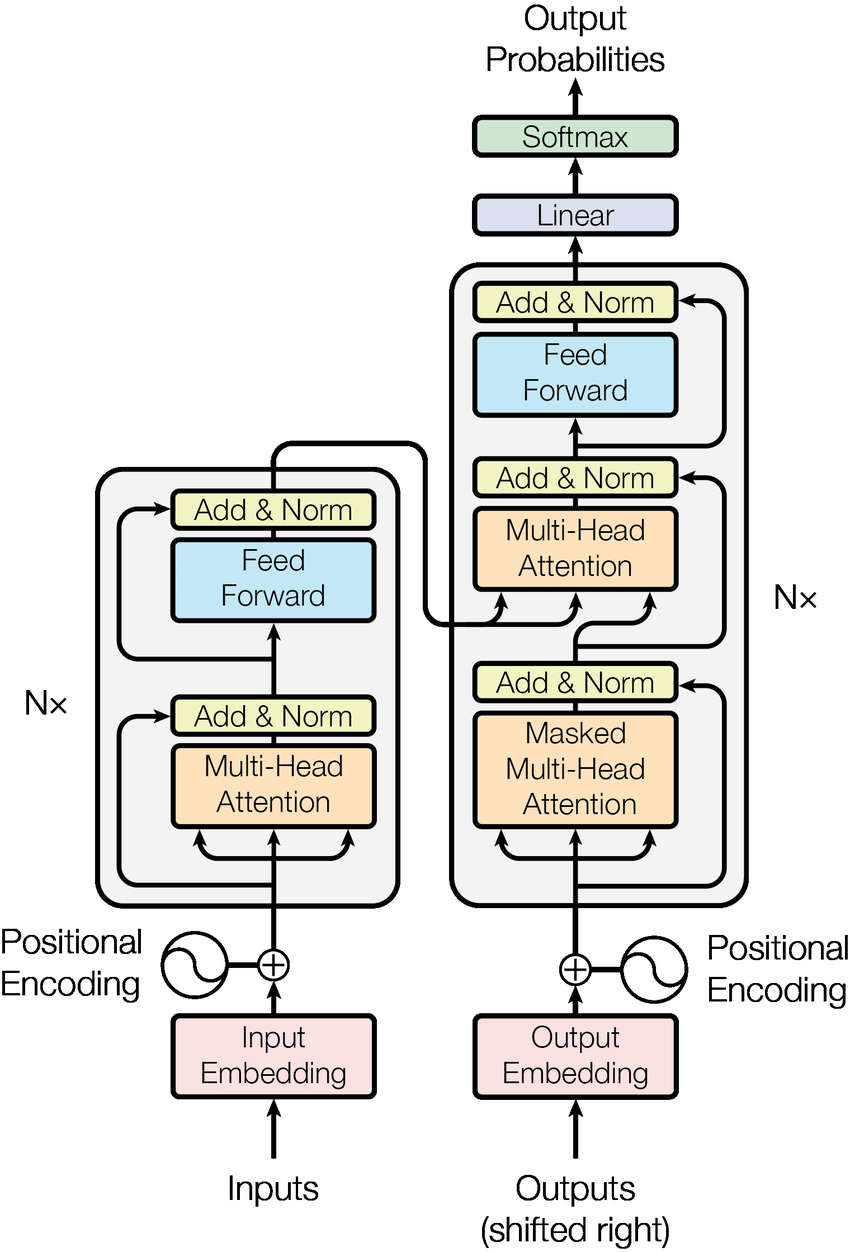
\includegraphics[width=0.85\columnwidth]{images/The-Transformer-model-architecture.png}
    \caption{The Transformer architecture by \citet{vaswani2017attention}.}
    \label{fig:transformer-architecture}
\end{figure}

\column{0.67\textwidth}

\textbf{Scaled Dot-Product Attention}

$W^Q \in \mathbb{R}^{d_{model} \times d_q}$, $W^K \in \mathbb{R}^{d_{model} \times d_k}$, $W^V \in \mathbb{R}^{d_{model} \times d_v}$. 

$Q = XW^{Q}$, $K = XW^{K}$, and $V = XW^{V}$.

$$Attention(Q, K, V) = softmax(\frac{QK^T}{\sqrt{d_k}})V$$

$$MultiHead Attention = Concat(head_1, ..., head_h)W^{O}$$

Where, $head_i = Attention(XW_{i}^{Q}, XW_{i}^{K}, XW_{i}^{V})$ and $W^O \in \mathbb{R}^{hd_v \times d_{model}}$.

\end{columns}

\end{frame}
%------------------------------------------------

%------------------------------------------------
%------------------------------------------------
\begin{frame}{Evaluation Tasks - Document Classification - MLDoc}

\begin{wideitemize}
    \item Assigning a document to a specific category based on its underlying semantic meaning. 
    \item The primary objective of Document Classification is to facilitate efficient information retrieval and management. 
    \item Spanish subset of MLDoc \citep{schwenk-li-2018-corpus}
    \begin{itemize}
        \item A comprehensive multilingual dataset comprising documents in eight languages.
        \item It is derived from the widely used Reuters Corpus \citep{reuters-DBLP:journals/jmlr/LewisYRL04}.
        \item Four distinct categories: Corporate/Industrial, Economics, Government/Social, and Markets.
    \end{itemize}
\end{wideitemize}

\end{frame}

%------------------------------------------------
\begin{frame}{Evaluation Tasks - Document Classification - MLDoc - Example}

\centering
\begin{figure}
    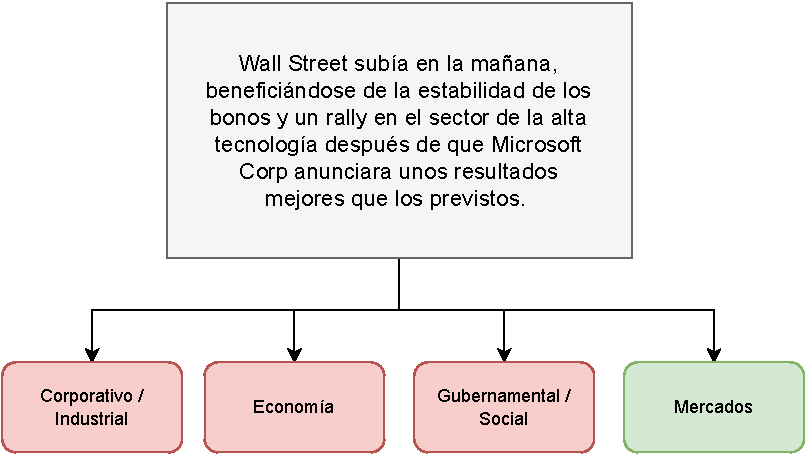
\includegraphics[scale=0.65]{images/nlp-example-document-classification.pdf}
    \caption{An example of document classification. Taken from the MLDoc \citep{schwenk-li-2018-corpus} dataset.}
    \label{fig:nlp-example-document-classification}
\end{figure}

\end{frame}
%------------------------------------------------
\begin{frame}{Evaluation Tasks - Paraphrase Identification - PAWS-X}

\begin{wideitemize}
    \item Determine whether two given sentences possess the same underlying semantic meaning.
    \item Spanish subset of PAWS-X \citep{yang-etal-2019-paws}
    \begin{itemize}
        \item It is a translation of the PAWS \citep{zhang-etal-2019-paws} dataset in six different languages.
        \item The training set of PAWS-X has been machine translated, while the validation and test sets were professionally translated by human experts.
    \end{itemize}
\end{wideitemize}

\end{frame}
%------------------------------------------------
\begin{frame}{Evaluation Tasks - Paraphrase Identification - PAWS-X - Example}

\centering
\begin{figure}
    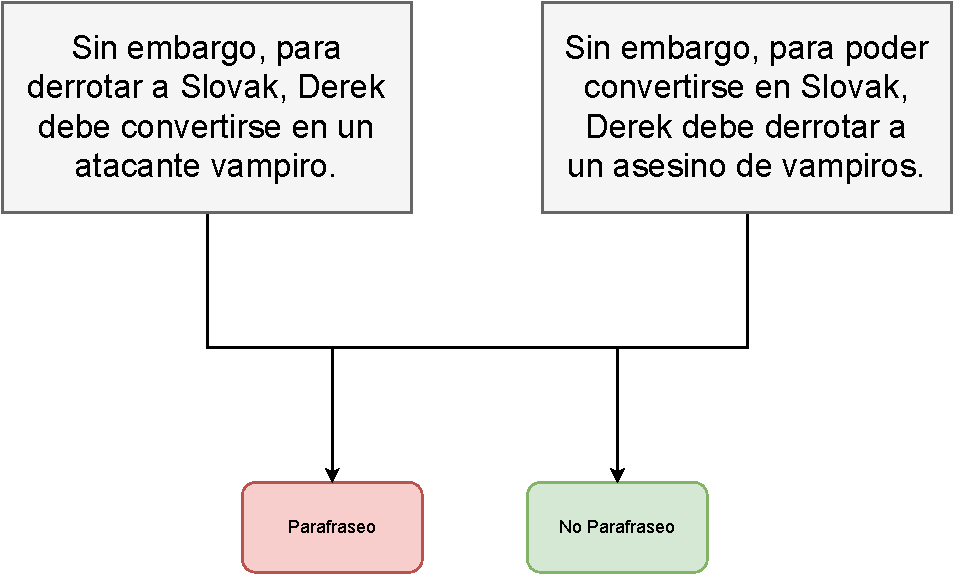
\includegraphics[scale=0.55]{images/nlp-example-paws-x.pdf}
    \caption{An example of the paraphrase identification task. Taken from the PAWS-X \citep{yang-etal-2019-paws} dataset.}
    \label{fig:nlp-example-paws-x}
\end{figure}

\end{frame}
%------------------------------------------------
\begin{frame}{Evaluation Tasks - Natural Language Inference - XNLI}

\begin{wideitemize}
    \item Determining the logical relationship between two given sentences, namely a "premise" and an "hypothesis". Specifically, the task requires inferring whether the premise entails, contradicts, or is neutral to the hypothesis.
    \item Spanish subset of XNLI \citep{conneau-etal-2018-xnli}
    \begin{itemize}
        \item It is a translation of the MultiNLI \citep{williams-etal-2018-broad} to 15 different languages.
        \item Offers a machine-translated training set while the validation and test sets have been professionally translated.
    \end{itemize}
\end{wideitemize}

\end{frame}
%------------------------------------------------
\begin{frame}{Evaluation Tasks - Natural Language Inference - XNLI - Example}

\centering
\begin{figure}
    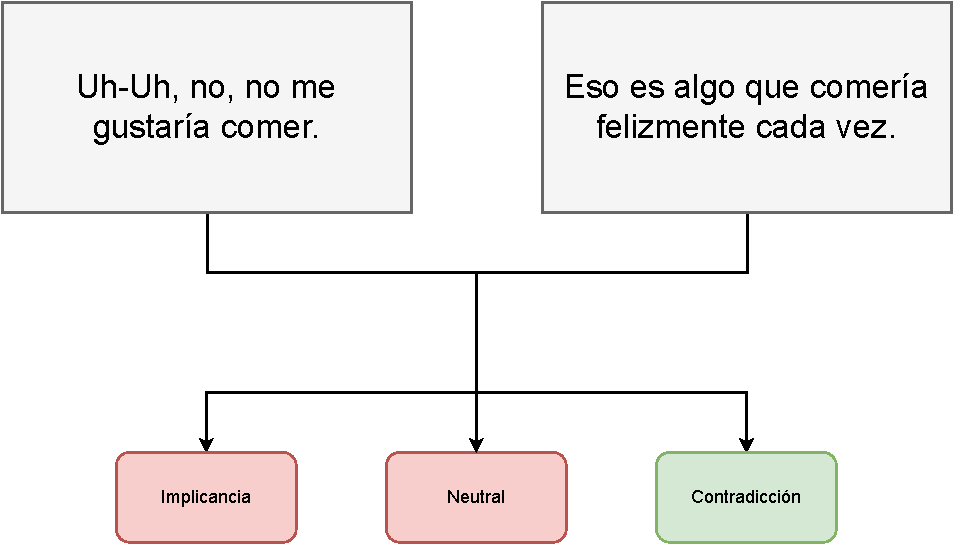
\includegraphics[scale=0.6]{images/nlp-example-xnli.pdf}
    \caption{An example of natural language inference. Taken from the XNLI \citep{conneau-etal-2018-xnli} dataset.}
    \label{fig:nlp-example-xnli}
\end{figure}


\end{frame}
%------------------------------------------------
\begin{frame}{Evaluation Tasks - Part-of-Speech Tagging - POS}

\begin{wideitemize}
    \item Task that aims to assign each word in a sentence its corresponding syntactic category.
    \item The syntactic categories are based on the grammatical function of the word and include, among others, nouns, verbs, adjectives, adverbs, and pronouns.
    \item The dataset used was AnCora \citep{taule-etal-2008-ancora} which is included on the Spanish part of Universal Dependencies \citep{de-marneffe-etal-2021-universal} Treebank.
\end{wideitemize}

\end{frame}
%------------------------------------------------
\begin{frame}{Evaluation Tasks - Part-of-Speech Tagging - POS - Example}

\centering
\begin{figure}
    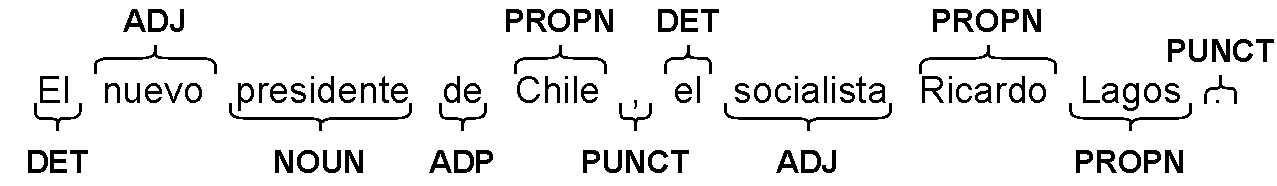
\includegraphics[width=\columnwidth]{images/nlp-example-pos.pdf}
    \caption{An example of the Part-of-Speech tagging task. Taken from the AnCora \citep{taule-etal-2008-ancora} dataset.}
    \label{fig:nlp-example-pos}
\end{figure}

\end{frame}
%------------------------------------------------
\begin{frame}{Evaluation Tasks - Named Entity Recognition - NER}

\begin{wideitemize}
    \item Involves identifying and classifying named entities within a text according to their corresponding types.
    \item It is essential in NLP as it enables computers to extract relevant information from unstructured text data, which can be used for a range of downstream applications.
    \item Named entities are typically classified into categories such as people, places, organizations, or miscellaneous entities.
    \item Entities may consist of multiple words. This complexity requires the adoption of the BIO annotation scheme in NER datasets, where each word is labeled as either the beginning (B) of an entity, inside (I) an entity, or outside (O) of any entity.
    \item Spanish subset of the CoNLL-2002 shared task dataset \citep{tjong-kim-sang-2002-introduction}.
\end{wideitemize}

\end{frame}
%------------------------------------------------
\begin{frame}{Evaluation Tasks - Named Entity Recognition - NER - Example}

\centering
\begin{figure}
    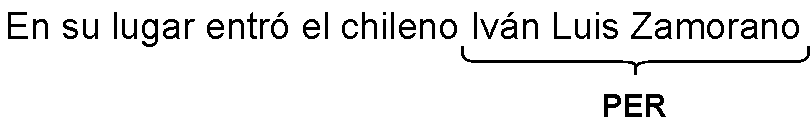
\includegraphics[width=\columnwidth]{images/nlp-example-ner.pdf}
    \caption{An example of named entity recognition. Taken from the CoNLL2002 NER \citep{tjong-kim-sang-2002-introduction} dataset.}
    \label{fig:nlp-example-ner}
\end{figure}

\end{frame}
%------------------------------------------------
\begin{frame}{Evaluation Tasks - Question Answering - MLQA - SQAC - TAR/XQuAD}

\begin{itemize}
    \item Extractive Question Answering: which aims to extract a span of words from a given context text that fully answers a question posed about that context.
    \item Spanish subset of MLQA \citep{lewis-etal-2020-mlqa}
    \begin{itemize}
        \item Multilingual dataset, created by translating English QA instances into 6 languages.
        \item The dataset provides a validation and a test set for each language, as well as a machine-translated version of the SQuAD v1.1 \citep{rajpurkar-etal-2016-squad} as a training set.
    \end{itemize}
    \item TAR \citep{carrino-etal-2020-automatic} + XQuAD \citep{artetxe-etal-2020-cross}
    \begin{itemize}
        \item TAR \citep{carrino-etal-2020-automatic} is another machine-translated dataset from SQuAD v1.1 to Spanish.
        \item XQuAD \citep{artetxe-etal-2020-cross} provides a test set that was obtained from SQuAD v1.1 and professionally translated into 11 different languages, including Spanish.
        \item Following the setup proposed by \citep{CaneteCFP2020}, we combined the train and validation sets from TAR and the Spanish test set from XQuAD as a single evaluation dataset.
    \end{itemize}
    \item SQAC \citep{gutierrezfandino2022-roberta-bne}
    \begin{itemize}
        \item May offer a more valuable resource for addressing Spanish language-related challenges, since it is the only one specifically designed for the Spanish language.
    \end{itemize}
\end{itemize}

\end{frame}
%------------------------------------------------
\begin{frame}{Evaluation Tasks - Question Answering - MLQA - SQAC - TAR/XQuAD - Example}

\centering
\begin{figure}
    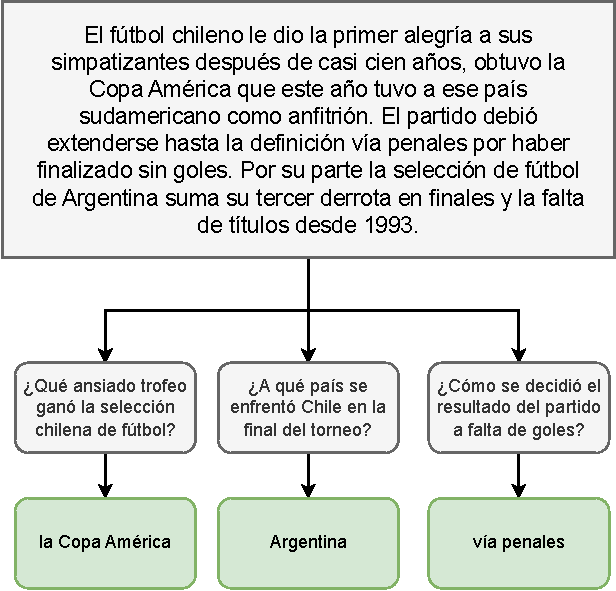
\includegraphics[scale=0.57]{images/nlp-example-question-answering.pdf}
    \caption{An example of question answering. Taken from the SQAC \citep{gutierrezfandino2022-roberta-bne} dataset.}
    \label{fig:nlp-example-question-answering}
\end{figure}

\end{frame}
%------------------------------------------------
\begin{frame}{Evaluation Metrics - Accuracy}

\textit{Accuracy} is a metric that calculates the ratio of correct predictions to the total number of predictions made by a model. It can be expressed mathematically as:

$$\text{Accuracy} = \frac{\text{Correct Predictions}}{\text{All Predictions}}$$

\end{frame}
%------------------------------------------------
\begin{frame}{Evaluation Metrics - F1 Score}

In the context of binary classification, \textit{Precision} is defined as the proportion of examples classified as positive that are truly positive. This can be expressed as:

$$\text{Precision} = \frac{\text{True Positives}}{\text{True Positives} + \text{False Positives}}$$

\textit{Recall} is defined as the proportion of truly positive examples that are correctly classified. This can be expressed as:

$$\text{Recall} = \frac{\text{True Positives}}{\text{True Positives} + \text{False Negatives}}$$

The \textit{F1 Score} is then defined as the harmonic mean of \textit{Precision} and \textit{Recall}, given by:

$$\text{F1 Score} = \frac{2 \cdot \text{Precision} \cdot \text{Recall}}{\text{Precision} + \text{Recall}}$$


\end{frame}
%------------------------------------------------
\begin{frame}{Evaluation Metrics - Exact Match}

In the case of Question Answering, the Exact Match metric compares the predicted answer string, $p_s$, with the correct answer string, $c_s$. The Exact Match for a single example is defined as:

\[
    \text{Exact Match}_{single} = 
\begin{cases}
    1, & \text{if } p_s == c_s\\
    0,              & \text{otherwise}
\end{cases}
\]

The Exact Match for a collection of pairs $(p_s, c_s) \in A$ is then defined as the average of the Exact Match for a single example, expressed as:

$$\text{Exact Match} = \sum_{(p_s, c_s) \in A} \frac{\text{Exact Match}_{single}(p_s, c_s)}{|A|}$$

\end{frame}
%------------------------------------------------
\begin{frame}{ALBETO - Dataset - SUC}

\begin{wideitemize}
    \item General domain corpora.
    \item Same corpus \citep{canete-compilation-corpora} used on BETO \citep{CaneteCFP2020}.
    \item 300M lines, 3B tokens, 18.4B chars.
    \item Sources: Spanish Wikis (dump of April 2019), Books, News, Subtitles, European Parliment, TED Talks, etc.
\end{wideitemize}

\end{frame}
%------------------------------------------------
\begin{frame}{ALBETO - Preprocessing}

\begin{wideitemize}
    \item Identical to BETO \citep{CaneteCFP2020} and very simple.
    \item Removing URLs and listings.
    \item Removing multiple whitespaces.
    \item Lowercase.
\end{wideitemize}

\end{frame}
%------------------------------------------------
\begin{frame}{ALBETO - Pre-training Details}

\begin{wideitemize}
    \item MLM and SOP.
    \item Single TPU v3-8 for each model.
    \item A maximum sequence length of 512 was used for pre-training, and the largest multiple of 64 that fit in the TPU memory was selected as the batch size.
    \item We experienced divergence in the loss on the \textit{large} and \textit{xlarge} models, this issue forced to stop the training and restart it from an earlier checkpoint with a slightly lower learning rate.
\end{wideitemize}

\begin{table}
\begin{center}
\resizebox{\textwidth}{!}{
\begin{tabular}{lcccccc}
\hline
\textbf{Model}          & \textbf{Learning Rate }  & \textbf{Batch Size} & \textbf{Warmup Ratio} & \textbf{Warmup Steps} & \textbf{Total Steps} & \textbf{Training Time (days)} \\ \hline
ALBETO \textit{tiny}    & 1.25e-3         & 2,048       & 1.25e-2       & 125,000       & 8,300,000     & 58.2                       \\ 
ALBETO \textit{base}    & 8.83e-4 & 960        & 6.25e-3      & 53,333        & 3,650,000     & 70.4                       \\ 
ALBETO \textit{large}   & 6.25e-4        & 512        & 3.12e-3     & 12,500        & 1,450,000     & 42.0                         \\ 
ALBETO \textit{xlarge}  & 3.12e-4       & 128        & 7.81e-4   & 6,250         & 2,775,000     & 64.2                       \\ 
ALBETO \textit{xxlarge} & 3.12e-4       & 128        & 7.81e-4   & 3,125         & 1,650,000     & 70.7                       \\ \hline
\end{tabular}}
\end{center}
\caption{Training details of all ALBETO models, which were trained using a single TPU v3-8 each one. }
\label{table:training-details-albetos}
\end{table}

\end{frame}
%------------------------------------------------
\begin{frame}{ALBETO - Training Loss - tiny}

\begin{figure}
    \centering
    \def\svgwidth{\columnwidth}
    \includesvg[]{loss_models/loss-albeto-tiny.svg}
    \caption{The progression of the training loss on the ALBETO \textit{tiny} model.}
    \label{fig:loss-albeto-tiny}
\end{figure}

\end{frame}
%------------------------------------------------
\begin{frame}{ALBETO - Training Loss - base}

\begin{figure}
    \centering
    \def\svgwidth{\columnwidth}
    \includesvg[]{loss_models/loss-albeto-base-2.svg}
    \caption{The progression of the training loss on the ALBETO \textit{base} model.}
    \label{fig:loss-albeto-base}
\end{figure}

\end{frame}
%------------------------------------------------
\begin{frame}{ALBETO - Training Loss - large}

\begin{figure}
    \centering
    \def\svgwidth{\columnwidth}
    \includesvg[]{loss_models/loss-albeto-large.svg}
    \caption{The progression of the training loss on the ALBETO \textit{large} model.}
    \label{fig:loss-albeto-large}
\end{figure}

\end{frame}
%------------------------------------------------
\begin{frame}{ALBETO - Training Loss - xlarge}

\begin{figure}
    \centering
    \def\svgwidth{\columnwidth}
    \includesvg[]{loss_models/loss-albeto-xlarge.svg}
    \caption{The progression of the training loss on the ALBETO \textit{xlarge} model.}
    \label{fig:loss-albeto-xlarge}
\end{figure}

\end{frame}
%------------------------------------------------
\begin{frame}{ALBETO - Training Loss - xxlarge}

\begin{figure}
    \centering
    \def\svgwidth{\columnwidth}
    \includesvg[]{loss_models/loss-albeto-xxlarge.svg}
    \caption{The progression of the training loss on the ALBETO \textit{xxlarge} model.}
    \label{fig:loss-albeto-xxlarge}
\end{figure}

\end{frame}
%------------------------------------------------
\begin{frame}{ALBETO - Fine-tuning Details}

\begin{itemize}
    \item We conducted a hyperparameter search on BETO, DistilBETO, RoBERTa-BNE, BERTIN, ALBETO \textit{tiny} and \textit{base}, exploring combinations of batch size \{16, 32, 64\}, learning rate \{1e-5, 2e-5, 3e-5, 5e-5\}, and number of epochs {2, 3, 4}.
    \item For the larger ALBETO models (\textit{large}, \textit{xlarge}, and \textit{xxlarge}), we reduced the learning rates to \{1e-6, 2e-6, 3e-6, 5e-6\} to mitigate numerical instability issues during training. 
    \item These fine-tuning procedures were performed on one to two NVIDIA RTX 3090 GPUs, depending on the model and task.
    \item To fine-tune the largest models on QA, we utilized two NVIDIA A100 GPUs from the Patagón supercomputer \cite{patagon-uach}.
    \item We used gradient accumulation in situations where the GPU memory was insufficient to reach the target batch size.
\end{itemize}

\end{frame}
%------------------------------------------------
\begin{frame}{Speedy Gonzales: KD Implementation - Text Classification - Single Sentence}

\begin{figure}
    \centering
    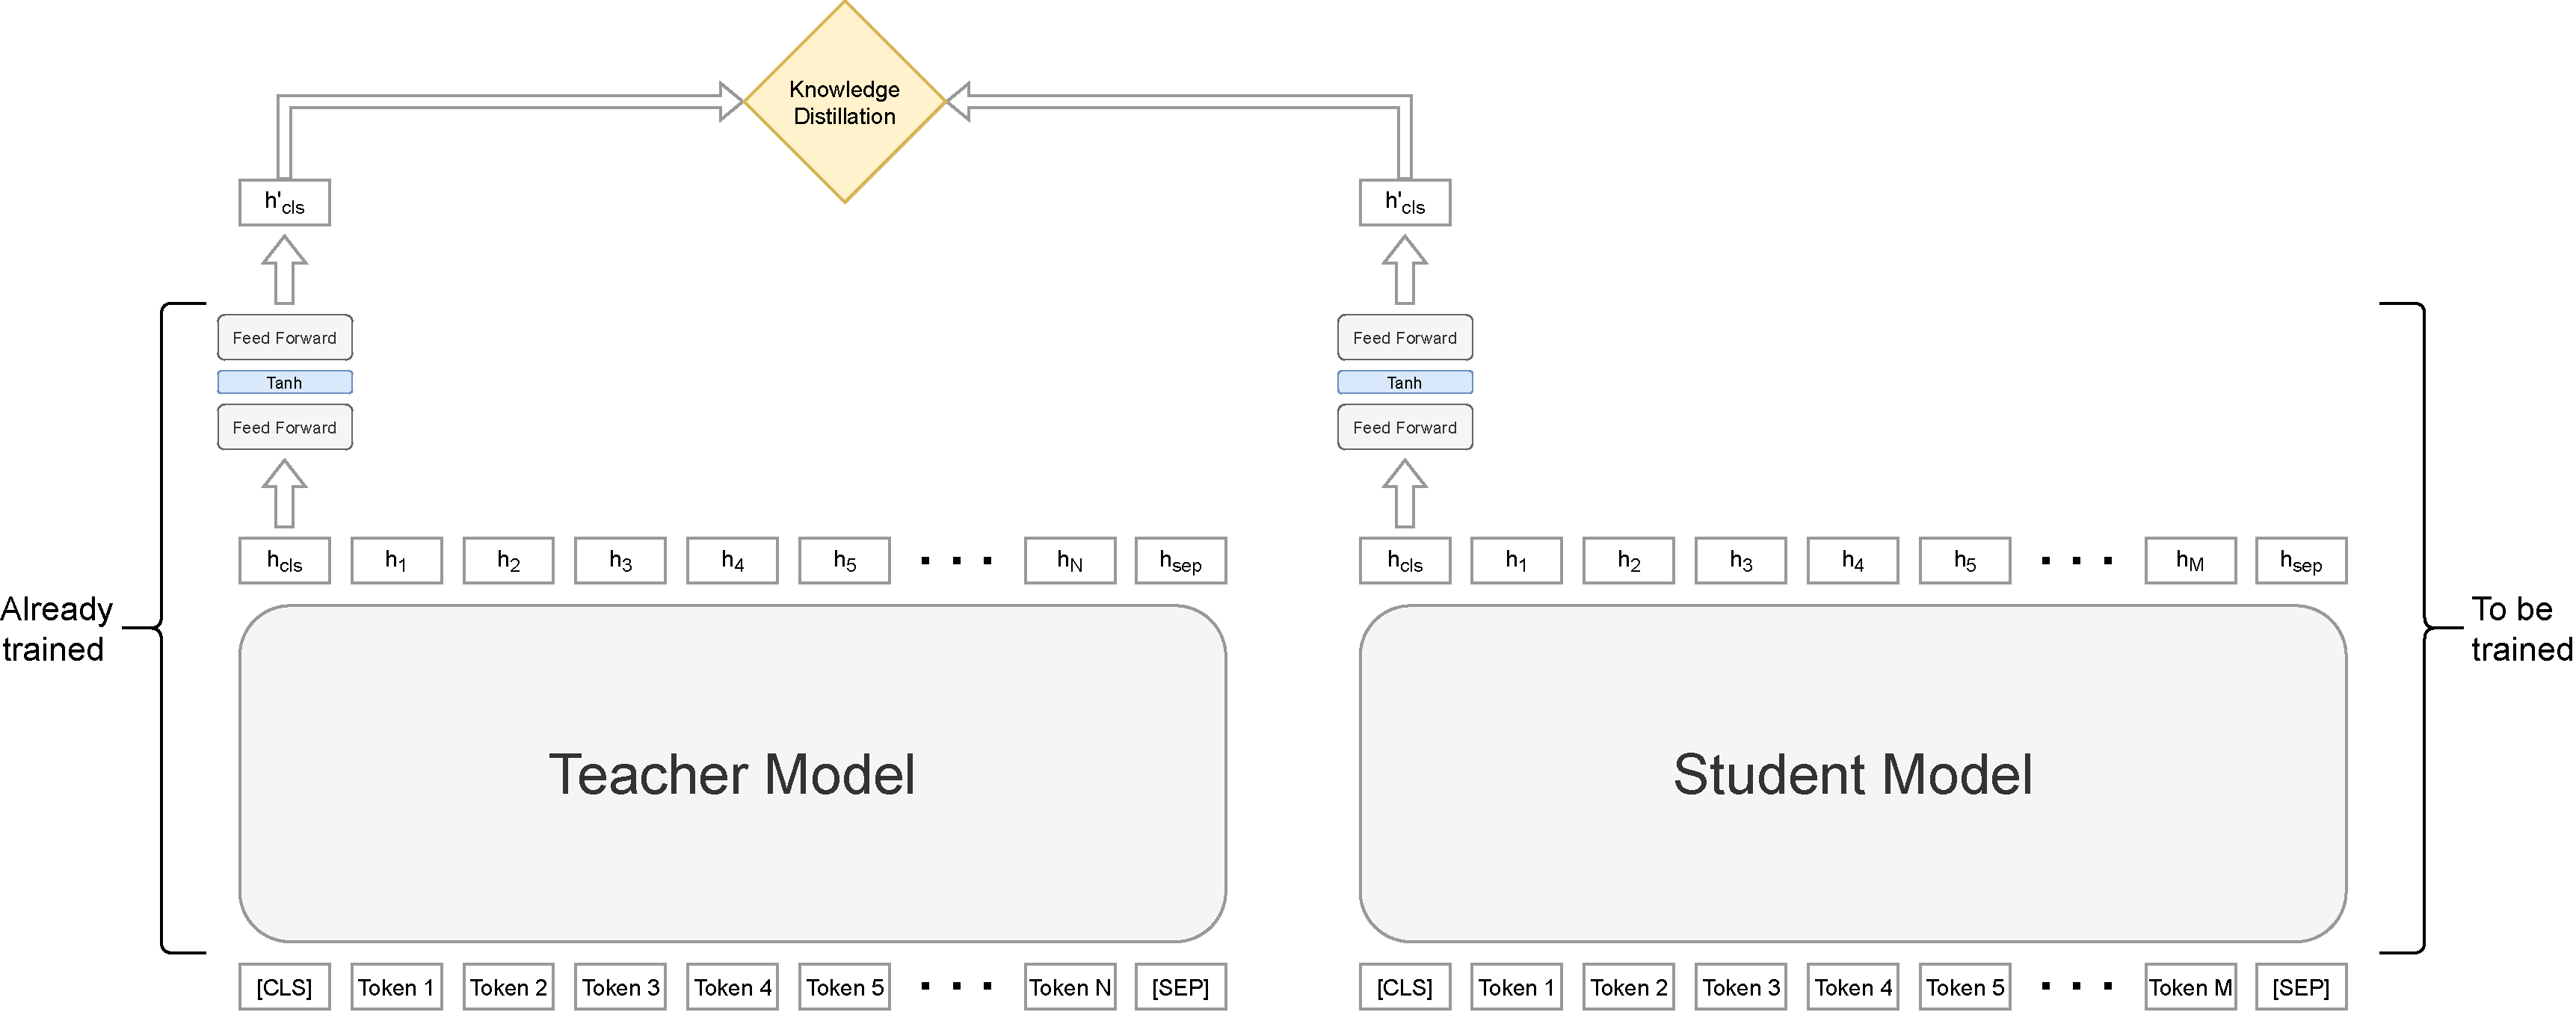
\includegraphics[width=\columnwidth]{images/single-sentence-text-classification-kd.pdf}
    \caption{Implementation of KD for text classifications tasks that use a single sentence as input.}
    \label{fig:single-sentence-text-classification-kd}
\end{figure}

\end{frame}
%------------------------------------------------
\begin{frame}{Speedy Gonzales: KD Implementation - Text Classification - Two Sentences}

\begin{figure}
    \centering
    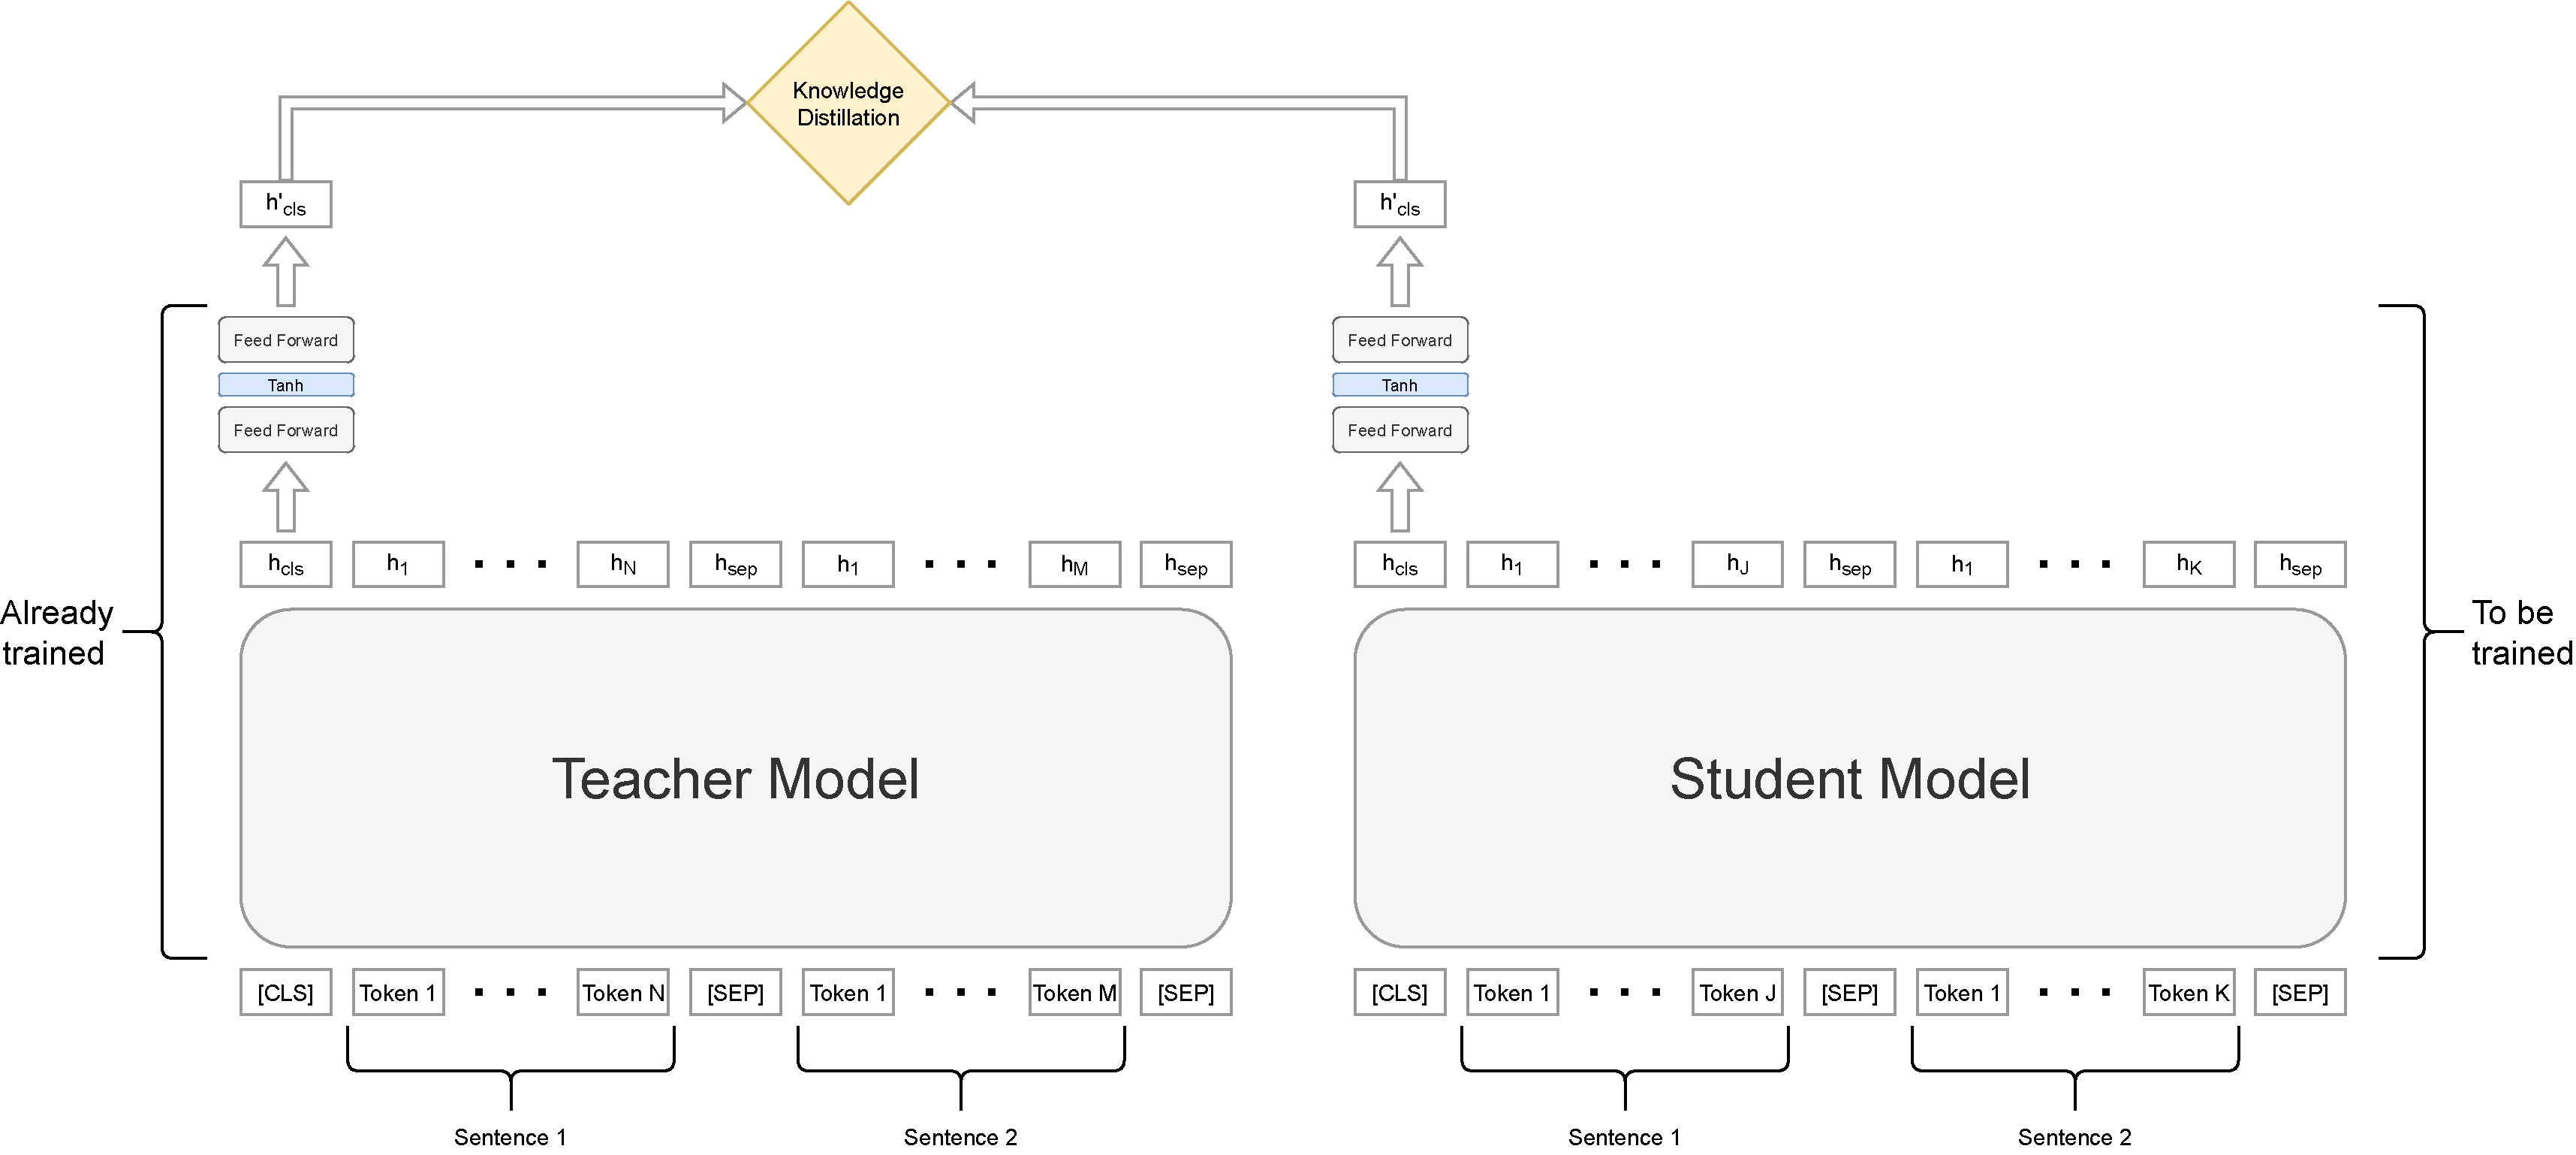
\includegraphics[width=0.88\columnwidth]{images/two-sentences-text-classification-kd.pdf}
    \caption{Implementation of KD for text classifications tasks that use two sentences as input.}
    \label{fig:two-sentences-text-classification-kd}
\end{figure}

\end{frame}
%------------------------------------------------
\begin{frame}{Speedy Gonzales: KD Implementation - Sequence Tagging}

\begin{figure}
    \centering
    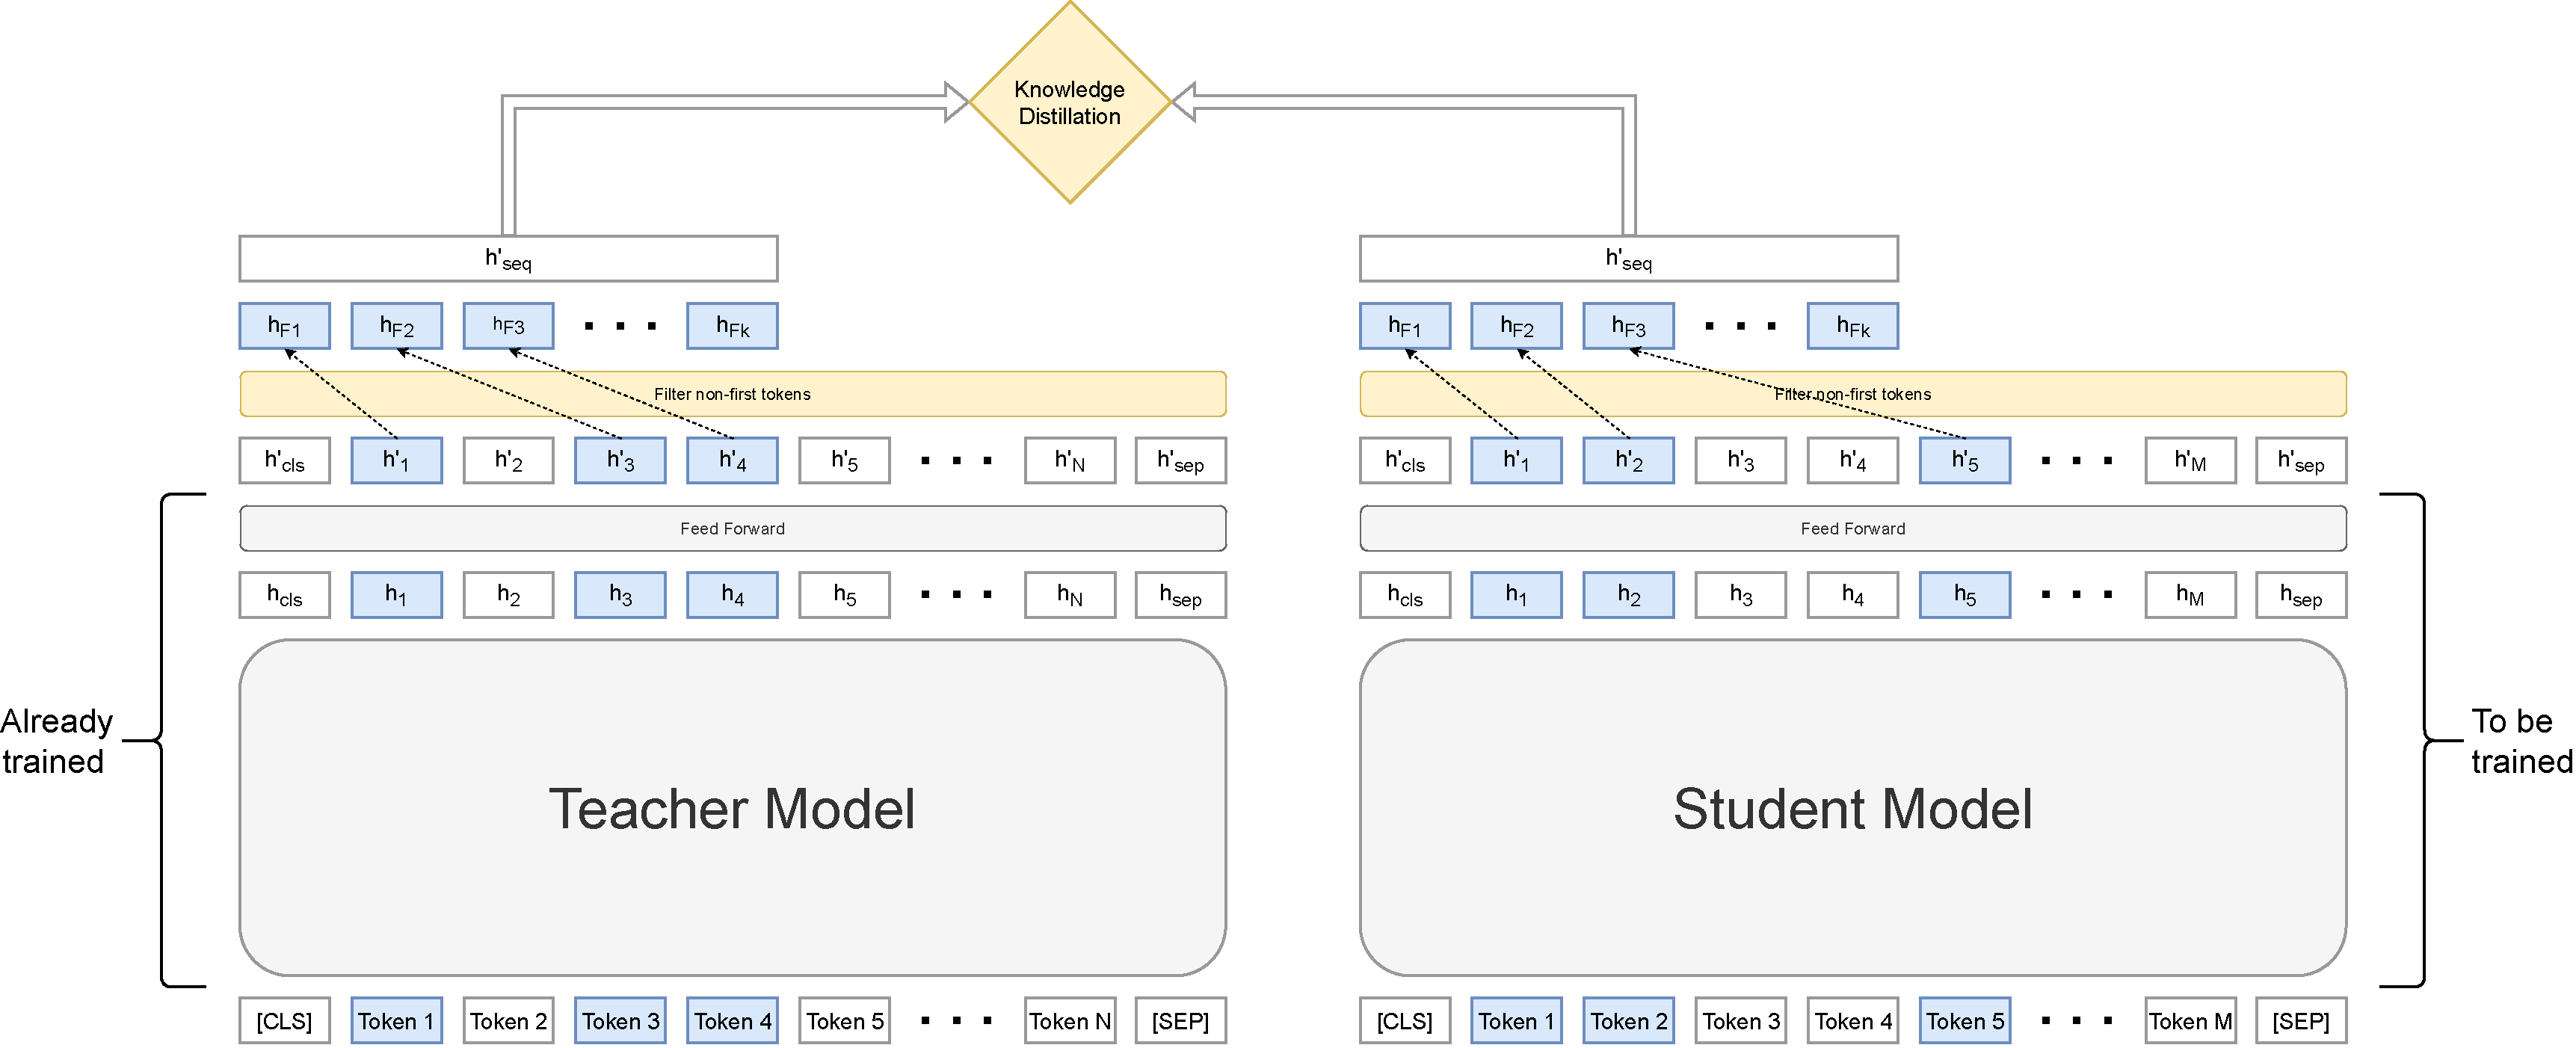
\includegraphics[width=0.9\columnwidth]{images/KD-sequence-tagging.pdf}
    \caption{Implementation of KD for sequence tagging tasks. The tokens marked with the blue color represents the property of being the first token of a word.}
    \label{fig:KD-sequence-tagging}
\end{figure}

\end{frame}
%------------------------------------------------
\begin{frame}{Speedy Gonzales: KD Implementation - Sequence Tagging - Same Vocabulary}

\begin{figure}
    \centering
    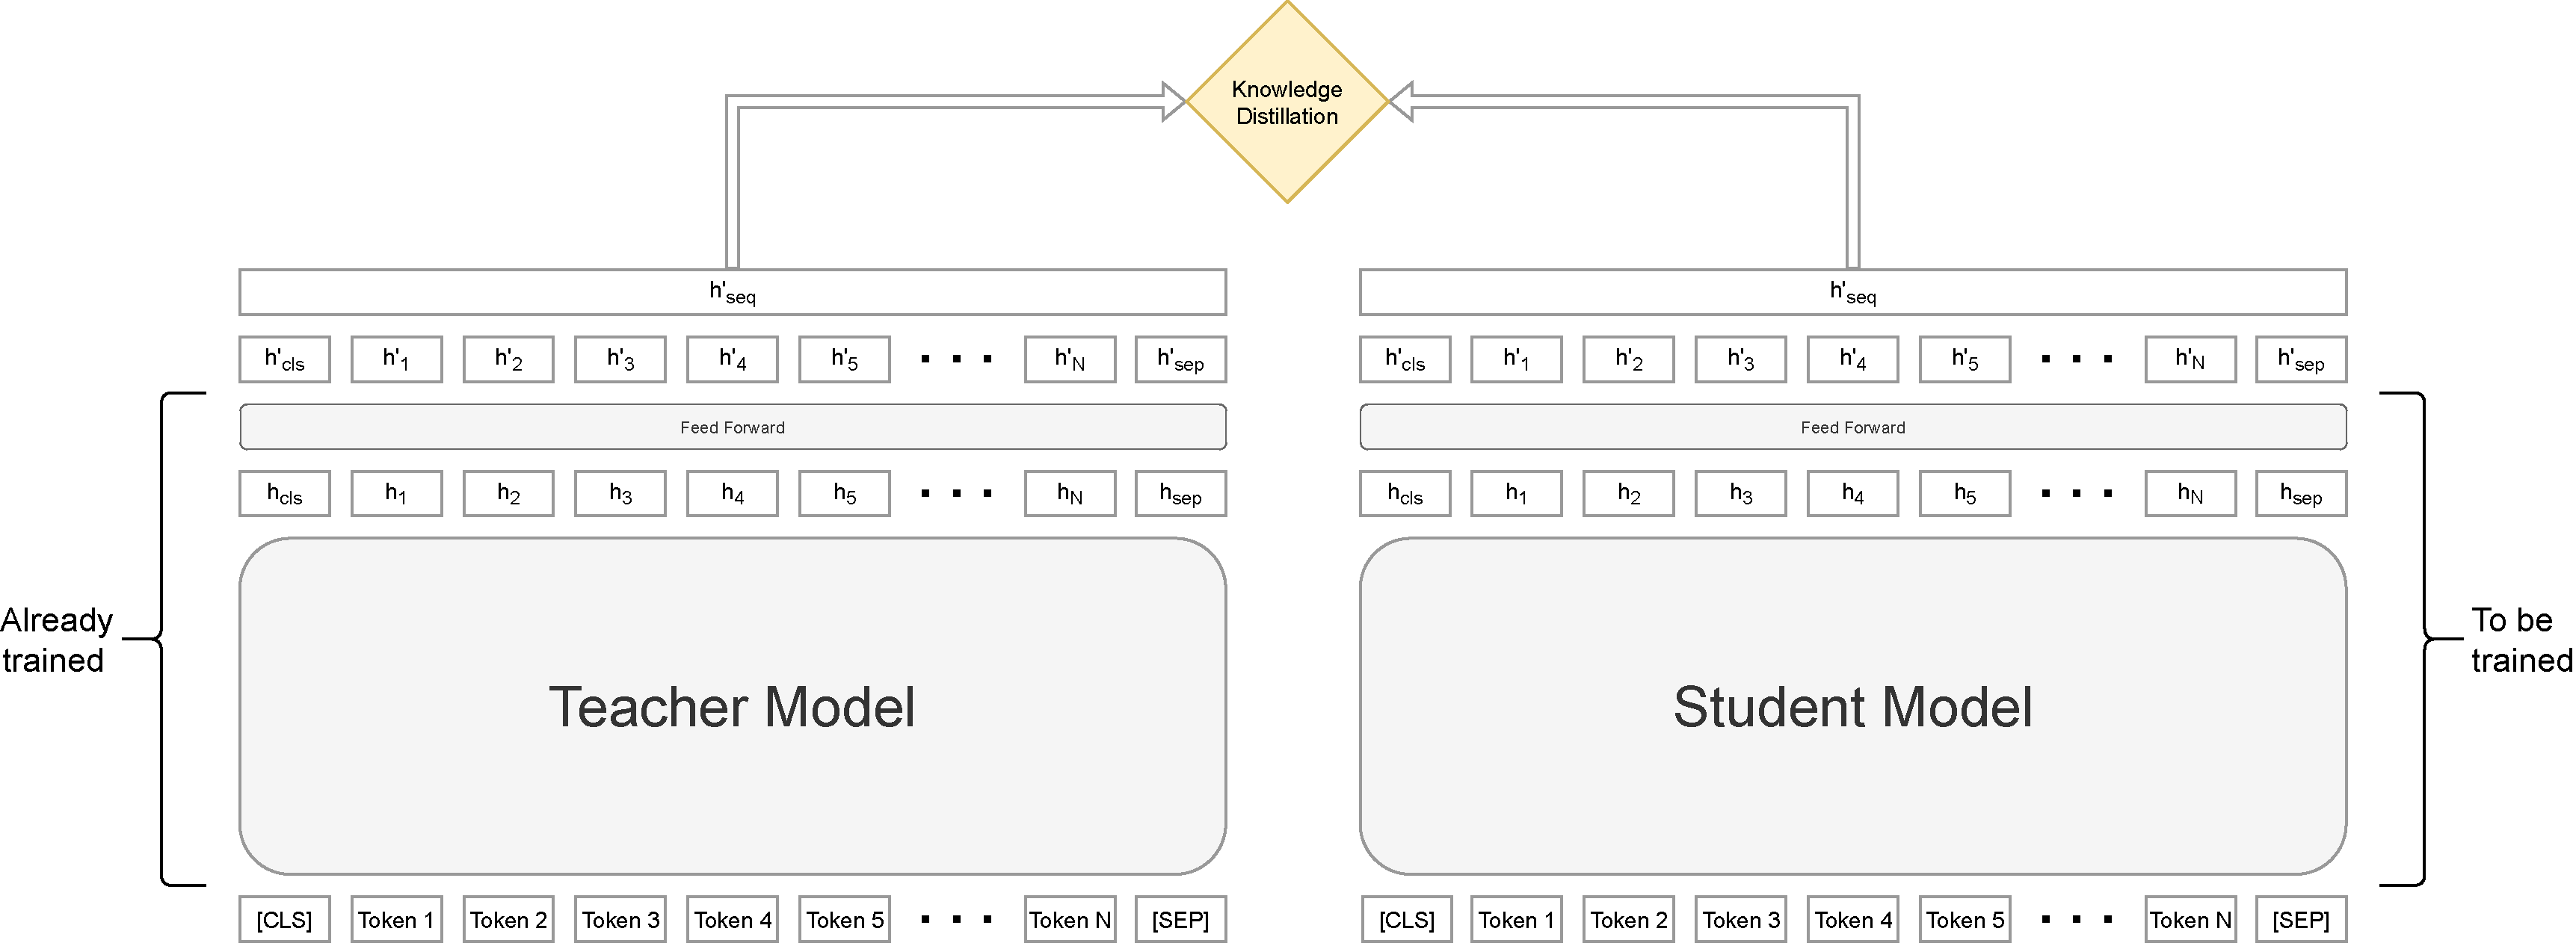
\includegraphics[width=\columnwidth]{images/KD-sequence-tagging-same-vocabulary.pdf}
    \caption{Implementation of KD for sequence tagging tasks with models that share the same vocabulary.}
    \label{fig:KD-sequence-tagging-same-vocabulary}
\end{figure}

\end{frame}
%------------------------------------------------
\begin{frame}{Speedy Gonzales: KD Implementation - Question Answering}

\begin{figure}
    \centering
    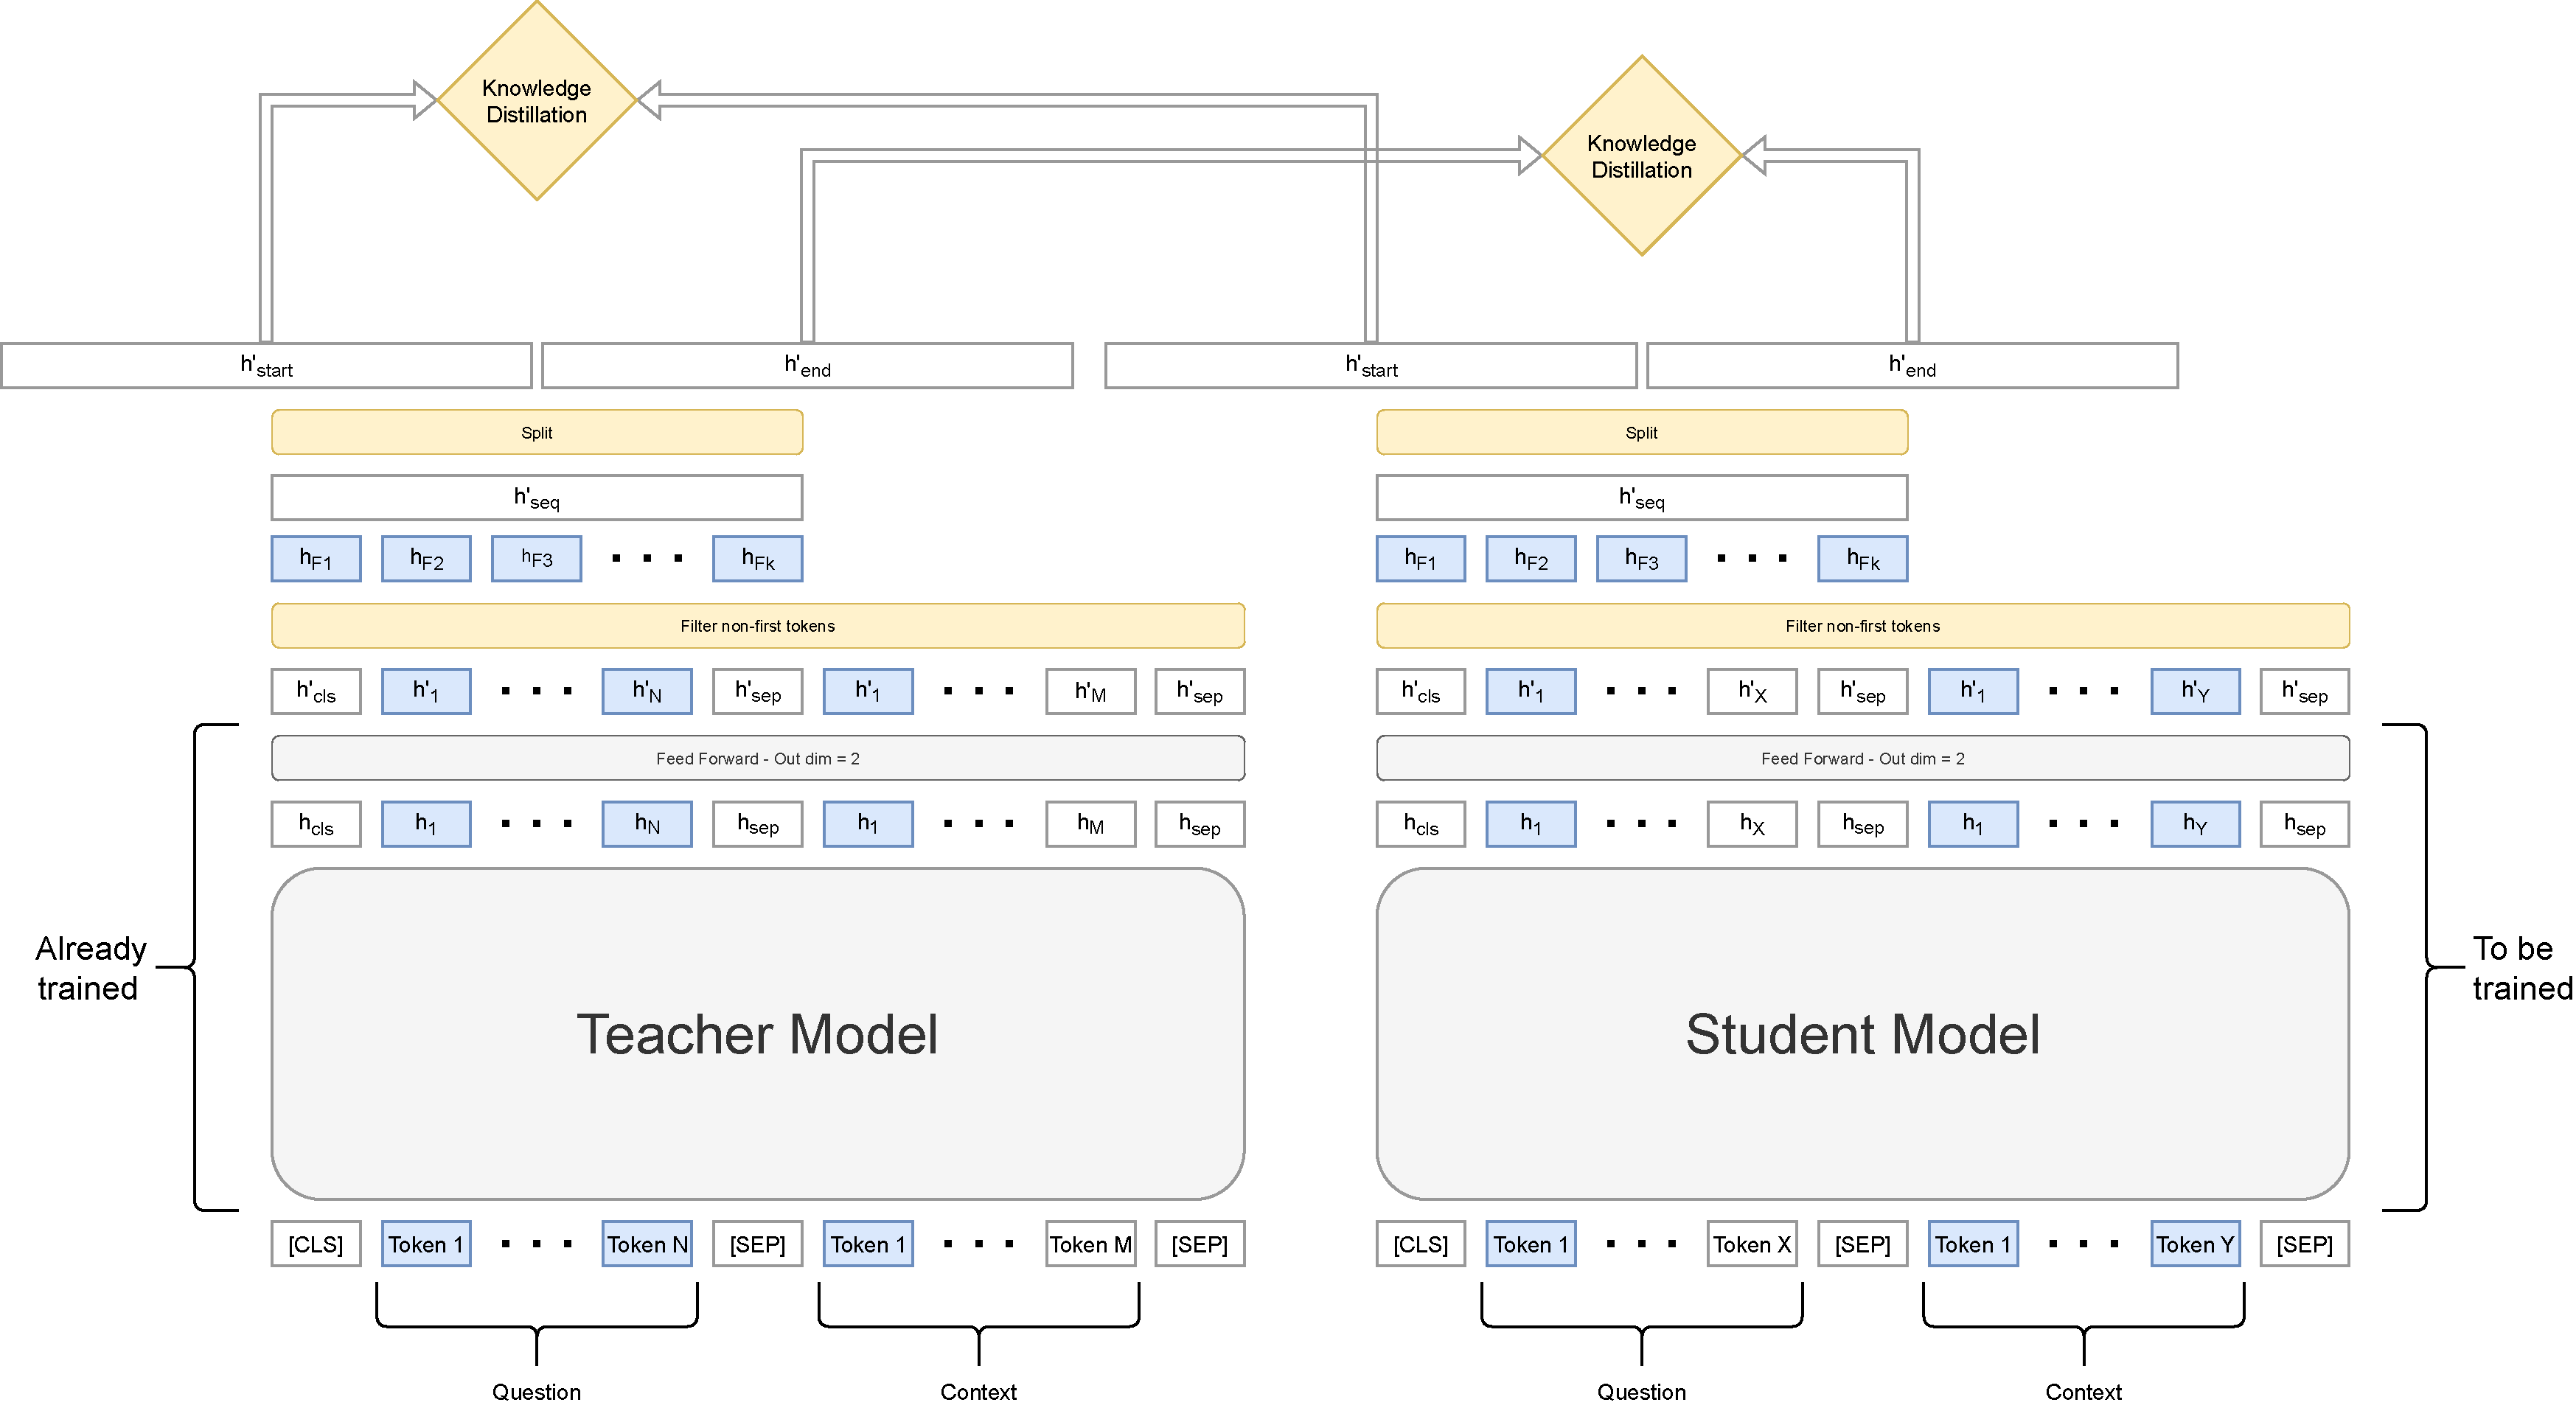
\includegraphics[width=0.69\columnwidth]{images/KD-QA.pdf}
    \caption{Implementation of KD for question answering datasets. The tokens marked with the blue color represents the property of being the first token of a word.}
    \label{fig:KD-QA}
\end{figure}


\end{frame}
%------------------------------------------------
\begin{frame}{Speedy Gonzales: KD Implementation - Question Answering - Same Vocabulary}

\begin{figure}
    \centering
    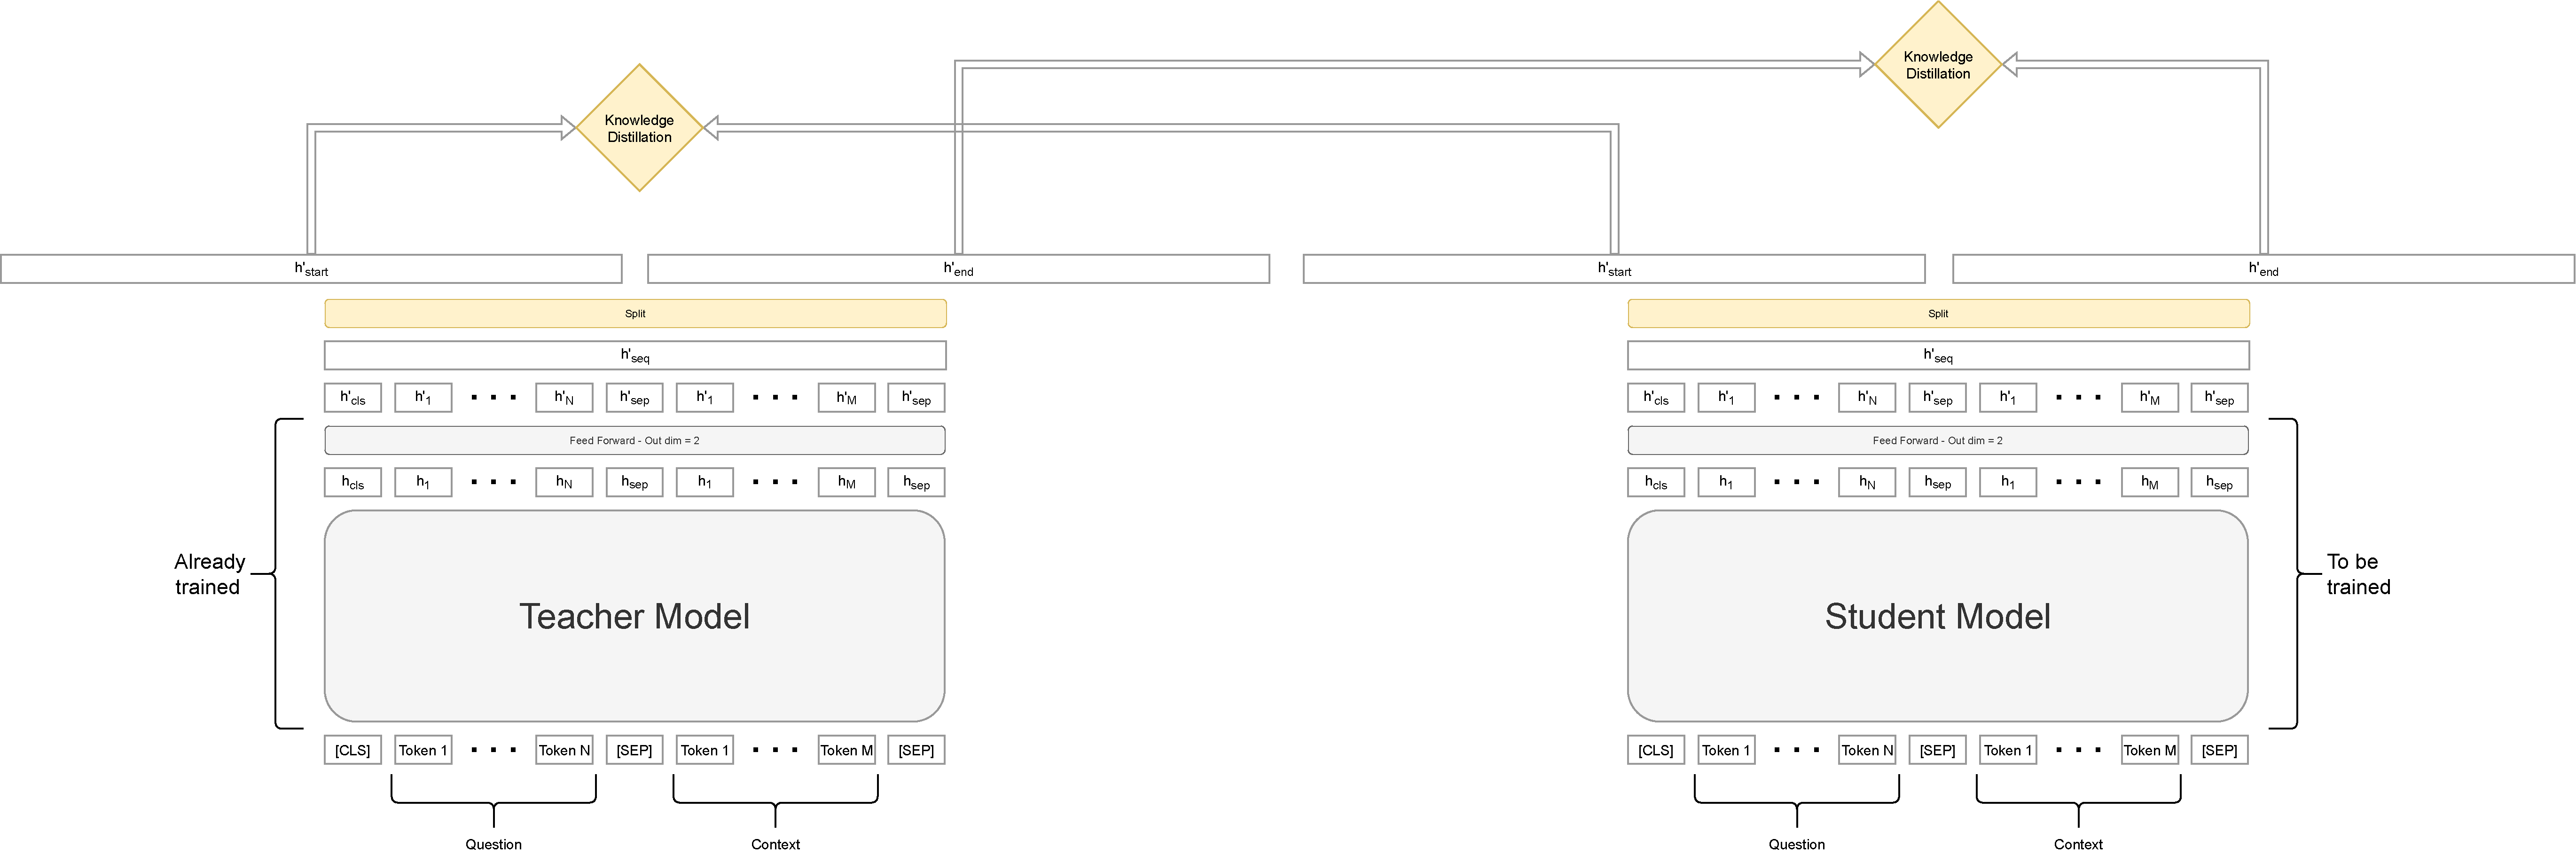
\includegraphics[width=\columnwidth]{images/KD-QA-same-vocabulary.pdf}
    \caption{Implementation of KD for question answering datasets with models that share the same vocabulary.}
    \label{fig:KD-QA-same-vocabulary}
\end{figure}

\end{frame}
%------------------------------------------------
\begin{frame}{Speedy Gonzales: Other details}

\begin{wideitemize}
    \item Our code uses Python and PyTorch \citep{pytorch-paper}.
    \item To measure MACs we used the THOP\footnote{\url{https://github.com/Lyken17/pytorch-OpCounter}} library.
    \item We conducted initial experiments utilizing three distinct loss functions: mean-squared error loss, cross-entropy loss, and KL-divergence loss. We varied the parameters $\alpha$ and $T$ across these losses using Optuna \citep{optuna-DBLP:conf/kdd/AkibaSYOK19}. The outcomes of these experiments revealed that the optimal settings were $\alpha = 0$ and $T = 1$. Although all three losses yielded satisfactory outcomes with this configuration, KL-divergence produced marginally superior results.
\end{wideitemize}

\end{frame}
%------------------------------------------------
\begin{frame}{Speedy Gonzales: Selected Teacher Models}

\begin{table}[]
\begin{center}
\begin{tabular}{ll}
\hline
\textbf{Dataset} & \textbf{Teacher Model} \\ \hline
MLDoc            & RoBERTa BNE \textit{large}      \\
PAWS-X           & ALBETO \textit{xxlarge}         \\
XNLI             & ALBETO \textit{xxlarge}         \\
POS              & RoBERTa BNE \textit{base}       \\
NER              & RoBERTa BNE \textit{base}       \\
MLQA             & ALBETO \textit{xxlarge}         \\
SQAC             & ALBETO \textit{xxlarge}         \\
TAR / XQuAD      & ALBETO \textit{xxlarge}        \\ \hline
\end{tabular}
\end{center}
\caption{The teacher models selected for each task.}
\label{table:selected-teacher-models}
\end{table}

Table \ref{table:selected-teacher-models} presents the teacher models selected for each task. The selection process is based on the lowest validation loss achieved among the candidate teacher models that were fine-tuned for each task.

\end{frame}
%------------------------------------------------






\begin{frame}[t, allowframebreaks]{Bibliography}
\bibliographystyle{plainnat}
\bibliography{bibliografia}
\end{frame}
%------------------------------------------------

\begin{frame}
    \titlepage
\end{frame}

%----------------------------------------------------------------------------------------


\end{document}